\newpage
\begin{appendices}
\iftoggle{toclinks}{\gototoc}{} % Turn it on/off in packages.tex, command in macros.tex
\iftoggle{cboxes}{	   				  % Turn it on/off in packages.tex
	\begin{boxeditems}
		\item Add link to website for Excel file with tickers.
		\item Add reference to paper that compares YC from Bloomberg for the Euro area.
	\end{boxeditems}}{}

\renewcommand\thefigure{\thesection.\arabic{figure}}
\section{Trend Inflation as a Proxy for Long-Term Inflation Forecasts} \label{sec:trendinf}
\setcounter{figure}{0}

An advantage of the small open economy approach is that it only requires forecasts for inflation, or a proxy in the case of countries with no long-term forecasts available as is the case for Israel and South Africa.

Inflation expectations are hoped to match measures of inflation that exclude unexpected shocks and better reflect the inflation environment.
Different measures of core inflation exist.
I use the inflation trend obtained by applying the Hodrick-Prescott filter to the series of realized inflation of each country.
Of course, the filter is sensitive to the sample period used.
The resulting trend can also be outside of the target inflation band due to the innate dynamics of the series, which would be at odds with survey data (see figure \ref{fig:wnCPI}).

%Fortunately, u
Unlike other countries, there is no marked upward or downward trend in the inflation of Israel nor South Africa during the sample period.
For each country, trend inflation is calculated for the whole period but only considered within the time range for which survey data is available for the rest of the countries, and as long as the trend is within the inflation target band.

Figure \ref{fig:CPI_ILSZAR} shows the realized and trend inflation for Israel and South Africa, and compares them with those of Malaysia and Thailand, two countries with a similar pattern for inflation (i.e. no marked trend) and for which survey data is available.
%It supports that t
Trend inflation seems to be a good proxy for the long-term inflation forecasts of Israel and South Africa.
Finally, since the 5-year and long-term forecasts closely follow each other (see figure \ref{fig:wnCPI}), I use trend inflation for both tenors.

\begin{landscape}
	\documentclass{article}
\usepackage{graphicx}
\usepackage[margin=1in]{geometry}
\usepackage[outdir=./]{epstopdf}  					% Avoids errors when input figures
\usepackage[labelsep=period,labelfont=bf]{caption}
%\usepackage{subcaption}

\begin{document}

\begin{figure}[tbph]
	\begin{center}
		\caption{Trend versus Long-Horizon Forecasts of Inflation}
		\label{fig:CPI_ILSZAR}
		\includegraphics[trim={0cm 0cm 0cm 0cm},clip,height=1\textheight,width=1.4\textwidth]{../Figures/Surveys/CPI_ILSZAR.eps} \\
	\end{center}
	% trim = {<left> <lower> <right> <upper>}
%	\vspace{-0.4cm} \caption*{\footnotesize{\textit{Notes}: Notes.}}
\end{figure}

\end{document}
\end{landscape}

%		\begin{figure}[!htbp]
		\begin{centering}
			\vspace{12.5mm}
			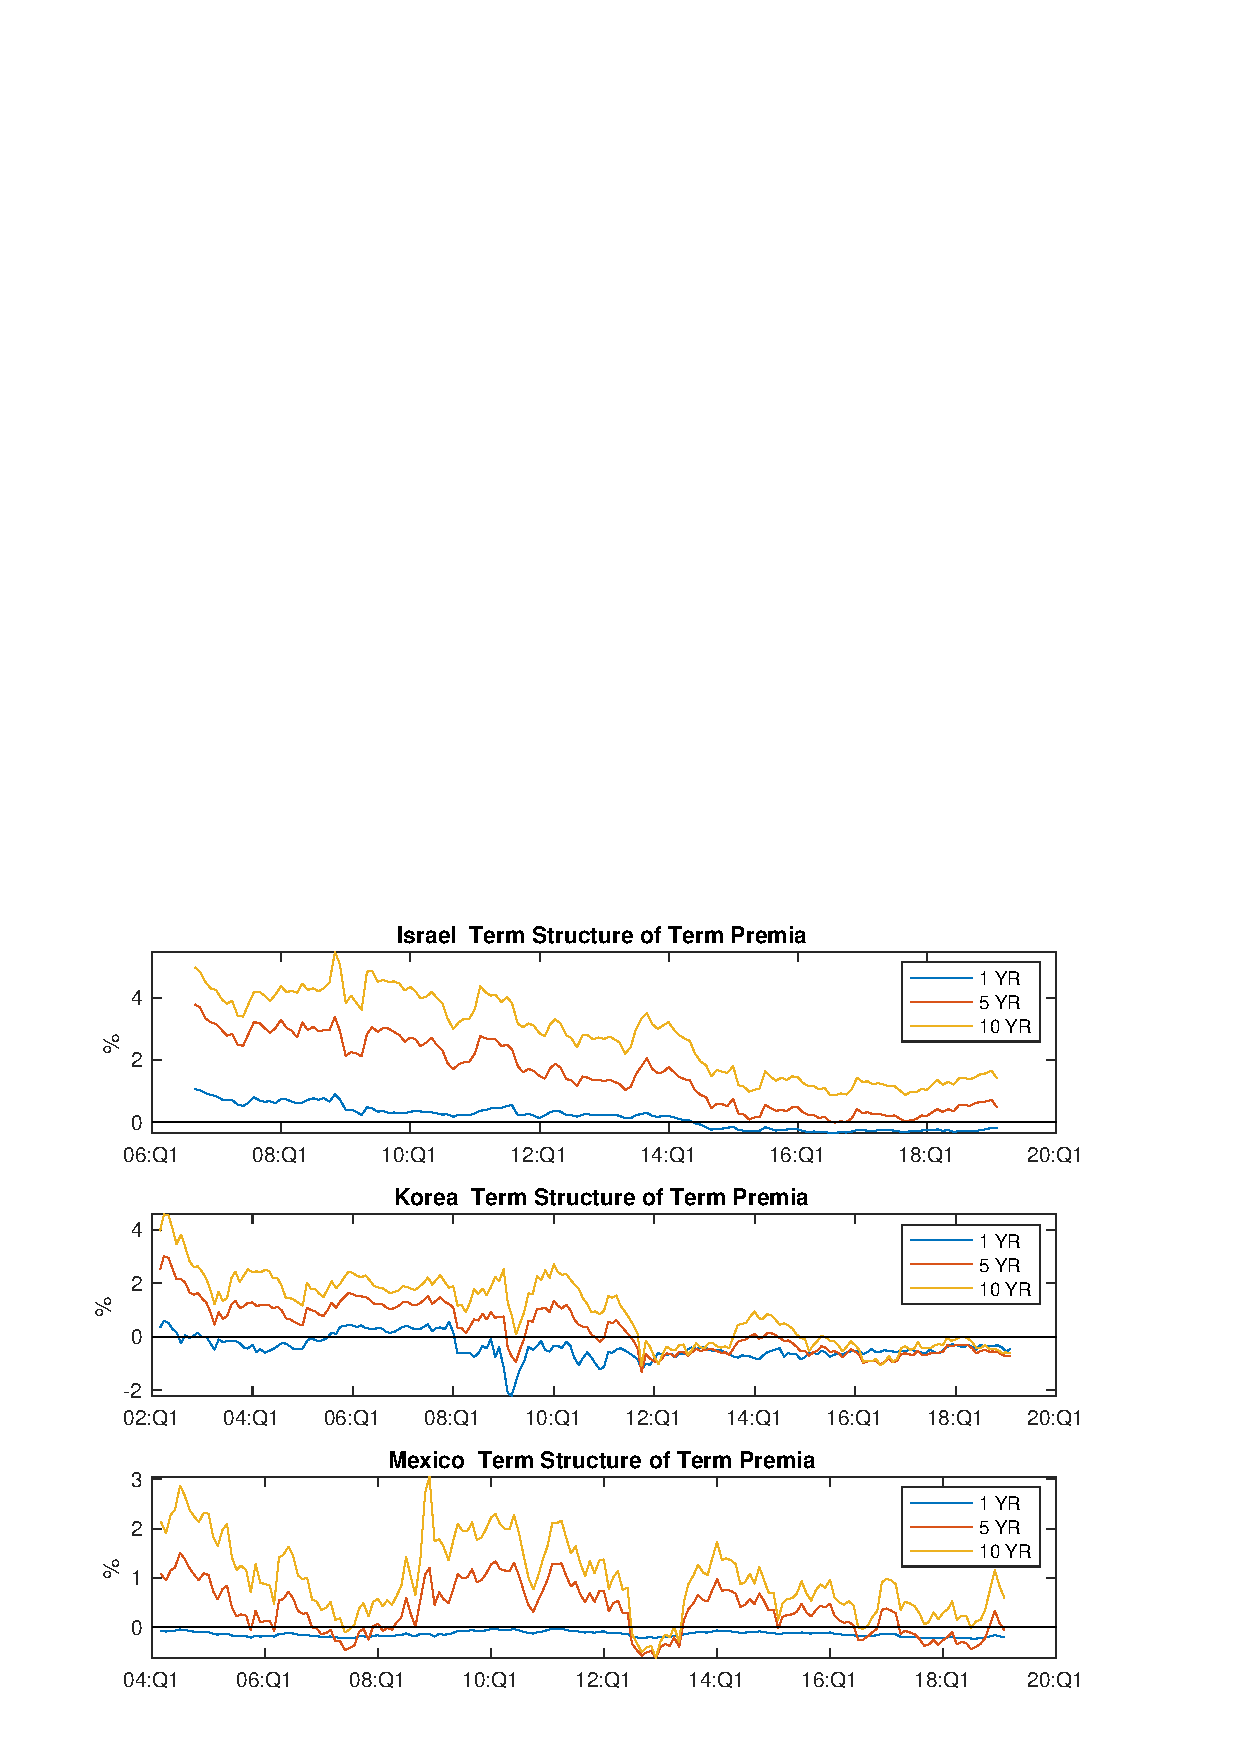
\includegraphics[width=1\textwidth,height=0.8\textheight]{../Figures/Temp/temp_ts_tp}
			\par\end{centering}
		\caption{Estimated Term Premia for Different Maturities.}\label{fig:temp_ts_tp}
	\end{figure}

\renewcommand\thefigure{\thesection.\arabic{figure}}
\section{Connectedness of Yield Components}
\setcounter{figure}{0}

%The expected short rate in emerging markets reacts to changes in the U.S. term premium. 
%This is consistent with the U.S. risk spillovers channel described by \cite{Kalemli-Ozcan:2019}.

%Here, I exploit it to provide new stylized facts about them that will help to interpret the results in the next section.
%To some extent, the response of emerging market yields to U.S. monetary policy shocks depends on 
%%how integrated are LC bonds to the global financial markets.
%%This requires to answer the question of 
%how connected are the sovereign yields of emerging markets.
%One way to address this question is to pool all yields together and see whether there is a global-level factor, associated with the first principal component.
%A global factor explains more than 90\% of the variation in the yields of advanced countries, 
%%consistent with \cite{DahlquistHasseltoft:2016}, 
%whereas it only explains around 50\% of the variation in the yields of emerging markets. % or their components.
%\footnote{ \cite{DuSchreger:2016JoF} find something similar for the credit risk compensation.}
%This suggests that the emerging market yields are not as connected among themselves as the yields of advanced countries.
%When yields are separated by maturity, a similar pattern emerges for the 1-year yields, whereas for the 10-year yields, a global factor explains around 95\% in AEs and 40\% in EMs. 
%Although a global factor plays a role in the variation of yields in both AEs and EMs, the bond yields in EMs are not as tightly connected as they are in AEs.
%These percentages are largely the same after the GFC.
%A global factor explains around 40\% of the variation of all the three components of yields in EMs.\footnote{ \cite{DuSchreger:2016JoF} also show that the credit risk compensation has a low reaction to global variables.} 
%For AEs, in contrast, a global factor explains 90\% of the variation in the expected short rate and 80\% in their term premia. 
%After the GFC, these percentages **increased** for the term premia in AEs and for the two components of the synthetic yields in EMs.

%A more formal way to analyze the comovement of %emerging market 
%%answer the question 
%yields is to measure the degree of connectedness among them.
%; that is, how much does the shock in one market has implications for the other markets.
%\cite{DieboldYilmaz:2014} propose a system-wide measure of connectedness 
%%based on forecast error variance decompositions.
%%Their methodology 
%that assesses shares of forecast error variation in a country's bond market due to shocks arising elsewhere.
%The connectedness index fluctuates between 0 and 100 percent, with higher numbers indicating a higher degree of comovement.
%Following \cite{ACDM:2019} and \cite{BostanciYilmaz:2020}, I obtain the connectedness index using a vector autoregression of order 1, with a forecast horizon of 10 days and a rolling window of 150 days for the daily changes of the 10-year nominal yield
%%of the emerging markets in the sample 
%and each of its components.

Figure \ref{fig:dyindex10y} shows that the connectedness index for the yields of emerging markets fluctuates around 30\%, %and advanced countries.
%\footnote{ The index for emerging markets has a shorter history because its computation requires a balanced panel. Also, since the construction of the synthetic curve does not involve nominal yields, the history of the components do not start on the same date.} 
%The index for emerging markets (figure \ref{subfig:dyindex10ydcmp}) captures some developments of the European sovereign debt crisis in 2012 and  the Greek debt crisis in 2015.
with notable spikes around the taper tantrum episode in 2013,
%\footnote{ During the episode, financial markets feared an earlier than expected withdrawal of the Fed's unconventional stimulus measures.} %and remained elevated for about a year.
%The second biggest spike %in the index occurred 
and after the 2016 U.S. presidential election.
%, with potential implications for some of the emerging markets in the sample.
%By mid-2017, the index was back to its pre-taper tantrum levels of around 30\% compared to an average value of the index for advanced countries of close to 70\%.
%The difference between the 
In contrast, \cite{ACDM:2019} report that the index fluctuates around 80\% for advanced countries.

The evidence of highly connected yields in advanced countries and low connected yields in emerging markets %might seem at odds with the idea of a 
%perspective based on the 
%global financial cycle \citep{Rey:2013}.
%On the one hand, the yields of advanced countries are highly connected among themselves (see figure \ref{subfig:dyindex10yAE}), which over the last decade has been driven by an increase in the connectedness of their term premia, as documented by \cite{ACDM:2019}.
%Changes in the compensation for risk in one advanced country not only spillover to other advanced countries but they have become increasingly important for the variation in their yields.
%On the other hand, the yields among emerging markets are not as connected as those in advanced countries (see figure \ref{subfig:dyindex10ydcmp}).
%The level of the index for emerging markets is about half the level of the index for advanced countries, it shows no upward trend for either their nominal yields or their components.\footnote{ \cite{ACDM:2019} already document that the increase in the connectedness of the yields of advanced countries has been driven by an increase in the connectedness of their term premia.}
% of emerging market yields do not show a clear trend, their relative importance seems to depend on the current economic environment.
%as might be expected under a perspective based on the global financial cycle. %according to the idea of the
%Is there a component that is more connected? 
%Unlike the rise in the connectedness of the term premium among advanced countries, 
%These results, however, are 
is consistent with a view %the global financial cycle 
in which global bond markets essentially operate under a core-periphery structure, in which the bond markets of advanced countries constitute the (highly interconnected) core and those of emerging markets represent the (less connected) periphery.
Countries in the periphery are in turn connected to the network mainly through countries in the core.\footnote{ The core-periphery structure has been shown to be a good description of different networks in economics and finance.} % \cite{CvP:2014} show, for example, that the interbank market operates under such a structure.
According to this view, shocks to emerging market yields are mainly idiosyncratic---reflected in less comovement---so
%figures \ref{subfig:dyindex10ydcmp} and \ref{subfig:dyindex10yAE} are measuring the connectedness of the periphery and the core, respectively.
%Therefore, 
what matters for them %emerging market yields 
are not spillovers originating in other emerging markets but in advanced countries.
%, which makes the argument of a global financial cycle stronger, not weaker.

The connectedness index for the yields of emerging markets shows no clear trend for either the nominal or synthetic yields nor their components. 
In contrast, \cite{ACDM:2019} document that the increase in the connectedness of the yields of advanced countries has been driven by an increase in the connectedness of their term premia.
Nevertheless, the term premia in emerging markets has been slightly more connected since 2013, whereas the credit risk compensation is relatively less connected (see figure \ref{subfig:dyindex10ydcmp}).
In fact, the level of the index for the synthetic yields tends to be higher than that for the nominal yields (see figure \ref{subfig:dyindex10ynomsyn}), suggesting that credit risk is indeed a more idiosyncratic component of the yields.

%Are the short and long end equally connected?
%Diebold-Yilmaz index for 2Y and 10Y to test Obsfeld vs K-O
%A related question is whether the connectedness of yields is the same throughout the term structure or whether some sections of the curves are more connected than others.
%%The role of a global factor seems to be different throughout the yield curve.
%\cite{Obstfeld:2015} 
%%shows that the effects of the global financial cycle are different at the short than at the long end of the yield curve. In particular, he 
%argues that long-term bonds are more globally connected than short term ones.
%On the other hand, \cite{Kalemli-Ozcan:2019} argues that short-term yields suffer more the effects of global influences.
%When yields are separated by maturity, a global factor explains around 50\% of the variation in the 1-year yields of EMs, compared to 90\% for AEs. 
%For the 10-year yields, a global factor explains around 60\% of the variability in EMs, relative to 95\% in AEs. 
%However, the role of the global factor is larger for the two components of the synthetic yield curve in the long end than for the short end.
%In sum, the role of a global component is larger for long-term yields and its components.
%Figure \ref{fig:dy_index_ts} plots the connectedness index for different maturities.
%It shows that the long end is relatively more connected than the short end, similar to what is observed for advanced countries, although this pattern became relevant for emerging markets after the taper tantrum episode.
%The figure also shows that the connectedness of the short end of the yield curves is similar between advanced and emerging markets.
%The difference in connectedness between the two groups of countries is therefore driven by the medium and long end of their yield curves.
%Although foreign participation in LC bond markets has increased, it is still mostly held by local investors, especially medium- and longer-term bonds as suggested by figure \ref{fig:dy_index_ts}, 
%%of emerging markets are far from being fully integrated in the global financial markets 
%and are therefore more responsive to local factors.
%In sum, while the yields of emerging markets are indeed globally connected, they are less so than the yields of advanced countries. 
%In particular, 
%Several factors can explain these patterns, including segmented markets, capital controls, home bias and regional differences.
%therefore seem to play a bigger role in the yields of EMs, and its components, than they do for AEs.

Finally, notice that the low connectedness among the yields of emerging markets supports estimating the term structure models for their yield curves separately (as it has been done in the paper) rather than jointly.

\documentclass{article}
\usepackage{graphicx}
\usepackage[margin=1in]{geometry}
\usepackage[outdir=./]{epstopdf}  					% Avoids errors when input figures
\usepackage[labelsep=period,labelfont=bf]{caption}
%\usepackage{subcaption}

\begin{document}
\begin{figure}[tbph]
\caption{Connectedness of Sovereign 10-Year Yields} \label{fig:dyindex10y}
\begin{center}
	\begin{minipage}{0.9\linewidth}
	\begin{center}
	\begin{subfigure}[t]{\linewidth}
			\includegraphics[trim={0cm 0cm 0cm 0cm},clip,height=0.34\textheight,width=\linewidth]{../Figures/Estimation/dy_index10y.eps} \\
			\vspace{-0.35cm}
			\caption{Emerging Markets} \label{subfig:dyindex10yEM}
			\vspace{0.4cm}
	\end{subfigure}
	
	\begin{subfigure}[t]{\linewidth}
			\includegraphics[trim={0cm 0cm 0cm 0cm},clip,height=0.34\textheight,width=\linewidth]{../Figures/Estimation/dy_index10y_AE.eps} \\
			\vspace{-0.35cm}
			\caption{Advanced Countries} \label{subfig:dyindex10yAE}
	\end{subfigure}
	\end{center}
	\fignotes{This figure plots the connected index of \cite{DieboldYilmaz:2014} for the 10-year nominal yields (solid line) of emerging markets and advanced countries. The figure also shows the index for each yield component. The yields of advanced countries are decomposed into an expected future short-term interest rate (line) and a term premium (line). The yields of emerging markets further have a credit risk premium (line). The index is obtained using a vector autoregression of order 1, with a forecast horizon of 10 days and a rolling window of 150 days for the daily changes of the 10-year nominal yields and each of their components. For emerging markets, the indexes have a shorter history because their computation requires a balanced panel; the indexes of the components do not start on the same date because the construction of the synthetic curves does not involve nominal yields.}
	\end{minipage}
\end{center}
\end{figure}
\end{document}
% trim = {<left> <lower> <right> <upper>} % appendix

%---------------------------------------------------------------
% Figures and Tables
%---------------------------------------------------------------
\renewcommand{\thetable}{\thesection.\arabic{table}}
\renewcommand\thefigure{\thesection.\arabic{figure}}
\section{Supplementary Tables} \label{sec:AppTables}
\setcounter{table}{0}

\documentclass[a4paper,12pt]{article}
\usepackage[labelsep=period,labelfont=bf]{caption}
\usepackage{multirow}
\usepackage{booktabs}
\usepackage{threeparttable}
\usepackage{pdflscape}
\usepackage{tabularx}
\usepackage[margin=1in]{geometry}
%% Personalized Macros
% Definitions, Equations, Table of Contents, Tables, Subcaptions, Paths, Text Fomats

%-------------------------------------------------------------------
% Variable Definitions
%-------------------------------------------------------------------
\providecommand{\tnr}{n}
\providecommand{\tnrfwd}{m}
\providecommand{\idxt}{t}
\providecommand{\idxi}{i}
\providecommand{\idxh}{h}
\providecommand{\idxs}{\idxt,\tnr}
\providecommand{\idxsfwd}{\tnr | \tnrfwd}
\providecommand{\idxsfwdt}{\idxt,\idxsfwd}
\providecommand{\idxspnl}{\idxi,\idxt}
\providecommand{\idxspnlfwd}{\idxi,{\idxt+\idxh}}
\providecommand{\idxspnllag}{\idxi,{\idxt-1}}
\providecommand{\idxspnllaglag}{\idxi,{\idxt-j}}
\providecommand{\fInst}{f_{\idxs}}
\providecommand{\yld}{y}
\providecommand{\xpc}{e}
\providecommand{\yZero}{\yld_{\idxs}}
\providecommand{\yZeroQ}{\yZero^{\Qmeasure}}
\providecommand{\yZeroP}{\yZero^{\Pmeasure}}
\providecommand{\yZeroE}{\yZero^{\xpc}}
\providecommand{\yZeroFwd}{\frate_{\idxsfwdt}}
\providecommand{\yZeroEfwd}{\yZeroFwd^{\xpc}}
\providecommand{\Pzero}{P_{\idxs}}
\providecommand{\Pzerolag}{P_{\idxt+1,\tnr-1}}
\providecommand{\srate}{i}
\providecommand{\shortrate}{\srate_{\idxt}}
\providecommand{\shortratelag}{\srate_{\idxt-1}}
\providecommand{\frate}{f}
\providecommand{\realrate}{r_{\idxs}}
\providecommand{\rateSvy}{\srate_{\idxs}^{survey}}
\providecommand{\SDF}{M_{\idxt+1}}
\providecommand{\SDFprod}{\ExpP \left[\Pi_{j=1} ^\tnr M_{\idxt+j}\right]}
\providecommand{\SDFsum}{\ExpQ \left[\exp \left(- \Sigma_{j=0} ^{\tnr-1} \srate_{\idxt+j} \right) \right]}
\providecommand{\Xvars}{X_{\idxt}}
\providecommand{\XvarsFwd}{X_{\idxt+1}}
\providecommand{\affineA}{A_{\tnr}}
\providecommand{\affineB}{B_{\tnr}}
\providecommand{\affineAfwd}{A_{\tnr + 1}}
\providecommand{\affineBfwd}{B_{\tnr + 1}}
\providecommand{\affineAQ}{\affineA^{\Qmeasure}}
\providecommand{\affineBQ}{\affineB^{\Qmeasure}}
\providecommand{\affineAP}{\affineA^{\Pmeasure}}
\providecommand{\affineBP}{\affineB^{\Pmeasure}}
\providecommand{\affineAe}{\affineA^{\xpc}}
\providecommand{\affineBe}{\affineB^{\xpc}}
\providecommand{\affineAeFwd}{A_{\idxsfwd}^{\xpc}}
\providecommand{\affineBeFwd}{B_{\idxsfwd}^{\xpc}}
\providecommand{\yLCnom}{\yld_{\idxs} ^{LC}}
\providecommand{\yLCsynt}{\widetilde{\yld}_{\idxs} ^{LC}}
\providecommand{\yUS}{y_{\idxs} ^{US}}
\providecommand{\yUSsynt}{\widetilde{\yld}_{\idxs} ^{US}}
\providecommand{\fx}{\mathit{s}}

% Math fonts
\providecommand{\Xdim}{\mathrm{K}}
\providecommand{\Ydim}{\mathrm{N}}
\providecommand{\Sdim}{\mathrm{S}}
\providecommand{\Normal}{\mathcal{N}}
\providecommand{\Pmeasure}{\mathbb{P}}
\providecommand{\Qmeasure}{\mathbb{Q}}
\providecommand{\Expec}{\mathrm{E}_{t}}
\providecommand{\ExpP}{\mathrm{E}^{\Pmeasure}_{t}}
\providecommand{\ExpQ}{\mathrm{E}^{\Qmeasure}_{t}}
\providecommand{\Svy}{S}
\providecommand{\yVec}{\mathbf{\yld}_{t}}
\providecommand{\ySVec}{\yVec^{\Svy}}
\providecommand{\Avec}{\mathbf{A}}
\providecommand{\Bvec}{\mathbf{B}}
\providecommand{\ASvec}{\mathbf{A}^{\Svy}}
\providecommand{\BSvec}{\mathbf{B}^{\Svy}}
\providecommand{\uVec}{\mathbf{u}_{t}}
\providecommand{\uSVec}{\mathbf{u}_{t}^{\Svy}}
\providecommand{\Svec}{\mathbf{\Sigma}}
\providecommand{\SyVec}{\mathbf{\Svec}_{Y}}
\providecommand{\SsVec}{\mathbf{\Svec}_{\Svy}}

% Greeks
\providecommand{\termprm}{\tau_{\idxs}}
\providecommand{\riskprice}{\lambda_{t}}
\providecommand{\lambdazero}{\lambda_{0}}
\providecommand{\lambdaone}{\lambda_{1}}
\providecommand{\fwdprm}{\rho_{\idxs}}
\providecommand{\CIPdev}{\phi_{\idxs}}
\providecommand{\deltazero}{\delta_{0}}
\providecommand{\deltaone}{\delta_{1}}
\providecommand{\error}{\nu_{t+1}}
\providecommand{\errorQ}{\error^{\Qmeasure}}
\providecommand{\errorP}{\error^{\Pmeasure}}
\providecommand{\XmuP}{\mu^{\Pmeasure}}
\providecommand{\XmuQ}{\mu^{\Qmeasure}}
\providecommand{\XSigma}{\Sigma}
\providecommand{\XPhiP}{\Phi^{\Pmeasure}}
\providecommand{\XPhiQ}{\Phi^{\Qmeasure}}
\providecommand{\betaLT}{\beta_{0}}
\providecommand{\betaST}{\beta_{1}}
\providecommand{\betaMTns}{\beta_{2}}
\providecommand{\betaMTnss}{\beta_{3}}
\providecommand{\tauNS}{\tau_{1}}
\providecommand{\tauNSS}{\tau_{2}}
\providecommand{\tnrTauNS}{\tnr/\tauNS}
\providecommand{\tnrTauNSS}{\tnr/\tauNSS}
\providecommand{\params}{\theta}
\providecommand{\Vasy}{\Omega}
\providecommand{\cmpnt}{\Psi}
\providecommand{\Jacobian}{\Gamma}
\providecommand{\Hessian}{\mathcal{H}_\params}
\providecommand{\asydstr}{\sqrt{\Ydim} \left( \widehat{\cmpnt} - \cmpnt \right) \xrightarrow[]{d} \Normal \left(0,\, \Jacobian \, \Vasy \, \Jacobian' \right)}
\providecommand{\sampleHjoint}{\frac{1}{\Ydim} \frac{\partial^{2} \ell_{\Ydim} (\widehat{\params})}{\partial \params \partial \params'}}
\providecommand{\sampleHindiv}{\frac{1}{\Ydim} \sum_{i = 1}^{\Ydim} \frac{\partial^{2} \log \mathit{f} (X_{i} | \widehat{\params})}{\partial \params \partial \params'}}

% Nelson-Siegel_Svensson
\providecommand{\loadSTnsFwd}{\exp\left(-\tnrTauNS \right)}
\providecommand{\loadSTnssFwd}{\exp\left(-\tnrTauNSS \right)}
\providecommand{\loadMTnsFwd}{\left(\tnrTauNS\right) \loadSTnsFwd}
\providecommand{\loadMTnssFwd}{\left(\tnrTauNSS\right) \loadSTnssFwd}
\providecommand{\loadSTnsZero}{\frac{1-\loadSTnsFwd}{\tnrTauNS}}
\providecommand{\loadSTnssZero}{\frac{1-\loadSTnssFwd}{\tnrTauNSS}}
\providecommand{\loadMTnsZero}{\left(\loadSTnsZero - \loadSTnsFwd \right)}
\providecommand{\loadMTnssZero}{\left( \loadSTnssZero - \loadSTnssFwd \right)}

%\providecommand{\}{}
% DELETE in a later revision
\providecommand{\Xmu}{\mu}
\providecommand{\XPhi}{\Phi}
\providecommand{\XmuStar}{\mu^{*}}
\providecommand{\XPhiStar}{\Phi^{*}}
\providecommand{\STrate}{r}
\providecommand{\rShort}{\STrate_{t}}
\providecommand{\rShortlag}{\STrate_{t-1}}
\providecommand{\ySvy}{\STrate_{\idxs}^{survey}}
\providecommand{\TPatsm}{tp_{\idxs}}

%-------------------------------------------------------------------
% Equations
%-------------------------------------------------------------------
\newcommand{\eqyLCsynt}{\yLCsynt = \yUS + \fwdprm}
\newcommand{\eqCIPdevDS}{\CIPdev = \yLCnom - \yLCsynt}
\newcommand{\eqCIPdevQ}{\CIPdev = \yLCnom - \yZeroQ}

\newcommand{\PzeroP}{\Pzero = \ExpP \left[ \SDF \Pzerolag \right]}
\newcommand{\PzeroQ}{\Pzero = \ExpQ \left[ \exp\left(- \shortrate\right) \Pzerolag \right]}

\newcommand{\eqXvarsFwdQ}{\XvarsFwd = \XmuQ + \XPhiQ \Xvars  + \XSigma \errorQ}
\newcommand{\eqshortrate}{\shortrate = \deltazero + \deltaone' \Xvars}
\newcommand{\eqyZeroP}{\yZeroP = \affineAP + \affineBP \Xvars}
\newcommand{\eqyZeroQ}{\yZeroQ = \affineAQ + \affineBQ \Xvars}
\newcommand{\eqTP}{\termprm = \yZeroQ - \yZeroP}
\newcommand{\eqXvarsFwdP}{\XvarsFwd = \XmuP + \XPhiP \Xvars  + \XSigma \errorP}
\newcommand{\eqriskprice}{\riskprice = \lambdazero + \lambdaone \Xvars}
\newcommand{\eqSDF}{\SDF = \exp\left( -\shortrate -\frac{1}{2} \riskprice' \riskprice - \riskprice' \errorP \right)}
%\newcommand{}{}

\newcommand{\eqpanelUCSV}{\tau_{\idxspnl} = \alpha_{\idxi} + \beta_{1} \sigma^{\pi}_{\idxspnl} + \beta_{2} g_{\idxspnl} + u_{\idxspnl}}
\newcommand{\eqpanelTPreg}{\yld_{\idxspnl} = \alpha_{\idxi} + \gamma_{1}' z^{1}_{\idxspnl} + \gamma_{2}' z^{2}_{\idxspnl} + u_{\idxspnl}}
\newcommand{\eqySvy}{\rateSvy = \frac{\widehat{\beta}_{0}}{1-\widehat{\beta}_{\srate}} + \frac{\widehat{\beta}_{{\pi}}}{1-\widehat{\beta}_{\srate}} \pi_{\idxs}^{survey} + \frac{\widehat{\beta}_{{g}}}{1-\widehat{\beta}_{\srate}} g_{\idxs}^{survey} }

\newcommand{\eqyFwd}{\yZeroFwd = \left( \tnrfwd \yld_{\idxt,\tnrfwd} - \tnr \yZero \right)/ \left( \tnrfwd - \tnr \right) }
\newcommand{\eqAeFwd}{\affineAeFwd = \left( \tnrfwd A_{\tnrfwd}^{\xpc}  - \tnr \affineAe \right)/ \left( \tnrfwd - \tnr \right) }
\newcommand{\eqBeFwd}{\affineAeFwd = \left( \tnrfwd B_{\tnrfwd}^{\xpc}  - \tnr \affineBe \right)/ \left( \tnrfwd - \tnr \right) }
\newcommand{\eqrrt}{\rateSvy = \pi^{CE survey}_{\idxs} + \realrate^{*} = \pi^{CE survey}_{\idxs} + \left( \srate^{SPF survey}_{\idxs} - \pi^{SPF survey}_{\idxs} \right) }


\newcommand{\eqyVecY}{\yVec = \Avec + \Bvec \Xvars + \SyVec \uVec}
\newcommand{\eqyVecS}{\ySVec = \ASvec + \BSvec \Xvars + \SsVec \uSVec}

% One shock at a time
%\newcommand{\eqpanelLP}{\yld_{\idxspnlfwd} - \yld_{\idxspnllag} = \alpha_{\idxh,\idxi} + \beta_{\idxh} \epsilon_{\idxt} + \gamma_{\idxh} \Delta \yld_{\idxspnllag} + \phi_{\idxh} \fx_{\idxspnllag}  + u_{\idxspnlfwd}}

% All shocks at once
\newcommand{\eqpanelLP}{\yld_{\idxspnlfwd} - \yld_{\idxspnllag} = \alpha_{\idxh,\idxi} + \sum^{3}_{j = 1} \beta^{j}_{\idxh} \epsilon^{j}_{\idxt} + \gamma_{\idxh} \Delta \yld_{\idxspnllag} + \eta_{\idxh} \fx_{\idxspnllag}  + u_{\idxspnlfwd}} 

\newcommand{\eqpanelLPlevels}{\yld_{\idxspnlfwd} = \alpha_{\idxh,\idxi} + \sum^{3}_{j = 1} \beta^{j}_{\idxh} \epsilon^{j}_{\idxt} + \sum^{2}_{j = 1} \gamma^{j}_{\idxh} \yld_{\idxspnllaglag} + \eta_{\idxh} \fx_{\idxspnllag}  + u_{\idxspnlfwd}} 
% \beta^{target}_{\idxh} \epsilon^{target}_{\idxt} + \beta^{path}_{\idxh} \epsilon^{path}_{\idxt} + \beta^{lsap}_{\idxh} \epsilon^{lsap}_{\idxt} 

%---------------------------------------------------------------
% Table of Contents
%---------------------------------------------------------------
% Link to ToC from section
\newcommand{\gototoc}{\vspace{-2cm} \null\hfill [\hyperlink{toc}{Go2ToC}] \newline}

% Link back to section from ToC
\newcommand{\maketoc}{
	\hypertarget{toc}{}
	\newpage
	\tableofcontents
	\vspace{2.5\bigskipamount} }

% Box with bullets for tasks to do in a section
\newenvironment{boxeditems}
	{\begin{tabular}{|p{\linewidth}|}
	\hline
	\begin{itemize}
	}
	{
	\end{itemize}
	\\ \hline
	\end{tabular} \\
	}

%---------------------------------------------------------------
% Tables: Estout Commands following Jörg Weber
%---------------------------------------------------------------
\newcommand{\sym}[1]{\rlap{#1}}

\let\estinput=\input	% define new input command to flatten the document

\newcommand{\estauto}[2]{
	\newcolumntype{C}{>{\centering\arraybackslash}X}
	\vspace{.75ex}{
%		\begin{tabularx}{1.4\textwidth}{l*{#2}C}
		\begin{tabularx}{0.95\linewidth}{l*{#2}C}
			\toprule
			\estinput{#1}
			\\ \bottomrule
			\addlinespace[.75ex]
		\end{tabularx}
	}
}

% Allow line breaks with \\ in specialcells
\newcommand{\specialcell}[2][c]{\begin{tabular}[#1]{@{}c@{}}#2\end{tabular}}

%---------------------------------------------------------------
% Subcaptions
%---------------------------------------------------------------
% Notes after figures following Jörg Weber
\newcommand{\figtext}[1]{
	\vspace{-1ex}
	\captionsetup{justification=justified,font=footnotesize}
	\caption*{#1}
%	\captionsetup{justification=raggedright,singlelinecheck=false,font=footnotesize}
%	\caption*{\hspace{6pt}\hangindent=1.5em #1}
}

\newcommand{\fignote}[1]{\figtext{\emph{Note:~}~#1}}
\newcommand{\fignotes}[1]{\figtext{\emph{Notes:~}~#1}}

% Notes after tables
\newcommand{\tabnote}[1]{
	\begin{tablenotes}[para,flushleft]
		\footnotesize \emph{Notes:~}~#1
	\end{tablenotes}
}

%---------------------------------------------------------------
% Paths
%---------------------------------------------------------------
%\newcommand*{\pathFigs}{../Figures}
%\input{pathFigs/fig1.tex}

%---------------------------------------------------------------
% Text Fomats
%---------------------------------------------------------------
%\newcommand{\txtbi}[1]{\textbf{\textit{#1}}}

%---------------------------------------------------------------
% Other
%---------------------------------------------------------------
%\newcommand\LL[1]{\multicolumn{2}{|l}{#1}}
%\newcommand\RR[1]{\multicolumn{2}{c|}{#1}}
%\newcommand\LR[1]{\multicolumn{2}{|c|}{#1}}
%\newcommand\LL[1]{\multicolumn{1}{|c}{#1}}
%\newcommand\RR[1]{\multicolumn{1}{c|}{#1}}
%\newcommand\LR[1]{\multicolumn{1}{|c|}{#1}}
\pagestyle{empty}

\begin{document}
	\begin{normalsize}
%		\begin{landscape}
			\begin{table}[!h]
				\begin{center}
					\caption{Drivers of the Emerging Market 5-Year Nominal Yield and Its Components} \label{tab:ycdcmp5y}
					\begin{threeparttable}
						\estauto{../Tables/f_ycdcmp5y.tex}{6}
						\tabnote{This table reports the estimated slope coefficients of panel data regressions of the 5-year nominal yield and its components (expected short rate, term premium and credit risk compensation) on selected explanatory variables. The sample includes monthly data for 15 emerging markets starting in 2000:1 and ending in 2019:1. The dependent variables are expressed in basis points. The explanatory variables are the U.S. term premium and the U.S. expected short rate according to \cite{KimWright:2005}  with the same maturity as the dependent variables, the policy rate, domestic inflation and unemployment, the standardized exchange rate (local currency per USD), the log of the Vix, the log of the U.S. and global economic policy uncertainty indexes based on \cite{BakerBloomDavis:2016}, the global economic activity index of \cite{Hamilton:2019}. Driscoll--Kraay standard errors in parenthesis; lag length up to which the residuals may be autocorrelated is indicated. *, **, *** asterisks respectively indicate significance at the 10\%, 5\% and 1\% level.}
					\end{threeparttable}
				\end{center}
			\end{table}
%		\end{landscape}
	\end{normalsize}
\end{document} % appendix
\documentclass[a4paper,12pt]{article}
\usepackage[labelsep=period,labelfont=bf]{caption}
\usepackage{multirow}
\usepackage{booktabs}
\usepackage{threeparttable}
\usepackage{pdflscape}
\usepackage{tabularx}
\usepackage[margin=1in]{geometry}
%% Personalized Macros
% Definitions, Equations, Table of Contents, Tables, Subcaptions, Paths, Text Fomats

%-------------------------------------------------------------------
% Variable Definitions
%-------------------------------------------------------------------
\providecommand{\tnr}{n}
\providecommand{\tnrfwd}{m}
\providecommand{\idxt}{t}
\providecommand{\idxi}{i}
\providecommand{\idxh}{h}
\providecommand{\idxs}{\idxt,\tnr}
\providecommand{\idxsfwd}{\tnr | \tnrfwd}
\providecommand{\idxsfwdt}{\idxt,\idxsfwd}
\providecommand{\idxspnl}{\idxi,\idxt}
\providecommand{\idxspnlfwd}{\idxi,{\idxt+\idxh}}
\providecommand{\idxspnllag}{\idxi,{\idxt-1}}
\providecommand{\idxspnllaglag}{\idxi,{\idxt-j}}
\providecommand{\fInst}{f_{\idxs}}
\providecommand{\yld}{y}
\providecommand{\xpc}{e}
\providecommand{\yZero}{\yld_{\idxs}}
\providecommand{\yZeroQ}{\yZero^{\Qmeasure}}
\providecommand{\yZeroP}{\yZero^{\Pmeasure}}
\providecommand{\yZeroE}{\yZero^{\xpc}}
\providecommand{\yZeroFwd}{\frate_{\idxsfwdt}}
\providecommand{\yZeroEfwd}{\yZeroFwd^{\xpc}}
\providecommand{\Pzero}{P_{\idxs}}
\providecommand{\Pzerolag}{P_{\idxt+1,\tnr-1}}
\providecommand{\srate}{i}
\providecommand{\shortrate}{\srate_{\idxt}}
\providecommand{\shortratelag}{\srate_{\idxt-1}}
\providecommand{\frate}{f}
\providecommand{\realrate}{r_{\idxs}}
\providecommand{\rateSvy}{\srate_{\idxs}^{survey}}
\providecommand{\SDF}{M_{\idxt+1}}
\providecommand{\SDFprod}{\ExpP \left[\Pi_{j=1} ^\tnr M_{\idxt+j}\right]}
\providecommand{\SDFsum}{\ExpQ \left[\exp \left(- \Sigma_{j=0} ^{\tnr-1} \srate_{\idxt+j} \right) \right]}
\providecommand{\Xvars}{X_{\idxt}}
\providecommand{\XvarsFwd}{X_{\idxt+1}}
\providecommand{\affineA}{A_{\tnr}}
\providecommand{\affineB}{B_{\tnr}}
\providecommand{\affineAfwd}{A_{\tnr + 1}}
\providecommand{\affineBfwd}{B_{\tnr + 1}}
\providecommand{\affineAQ}{\affineA^{\Qmeasure}}
\providecommand{\affineBQ}{\affineB^{\Qmeasure}}
\providecommand{\affineAP}{\affineA^{\Pmeasure}}
\providecommand{\affineBP}{\affineB^{\Pmeasure}}
\providecommand{\affineAe}{\affineA^{\xpc}}
\providecommand{\affineBe}{\affineB^{\xpc}}
\providecommand{\affineAeFwd}{A_{\idxsfwd}^{\xpc}}
\providecommand{\affineBeFwd}{B_{\idxsfwd}^{\xpc}}
\providecommand{\yLCnom}{\yld_{\idxs} ^{LC}}
\providecommand{\yLCsynt}{\widetilde{\yld}_{\idxs} ^{LC}}
\providecommand{\yUS}{y_{\idxs} ^{US}}
\providecommand{\yUSsynt}{\widetilde{\yld}_{\idxs} ^{US}}
\providecommand{\fx}{\mathit{s}}

% Math fonts
\providecommand{\Xdim}{\mathrm{K}}
\providecommand{\Ydim}{\mathrm{N}}
\providecommand{\Sdim}{\mathrm{S}}
\providecommand{\Normal}{\mathcal{N}}
\providecommand{\Pmeasure}{\mathbb{P}}
\providecommand{\Qmeasure}{\mathbb{Q}}
\providecommand{\Expec}{\mathrm{E}_{t}}
\providecommand{\ExpP}{\mathrm{E}^{\Pmeasure}_{t}}
\providecommand{\ExpQ}{\mathrm{E}^{\Qmeasure}_{t}}
\providecommand{\Svy}{S}
\providecommand{\yVec}{\mathbf{\yld}_{t}}
\providecommand{\ySVec}{\yVec^{\Svy}}
\providecommand{\Avec}{\mathbf{A}}
\providecommand{\Bvec}{\mathbf{B}}
\providecommand{\ASvec}{\mathbf{A}^{\Svy}}
\providecommand{\BSvec}{\mathbf{B}^{\Svy}}
\providecommand{\uVec}{\mathbf{u}_{t}}
\providecommand{\uSVec}{\mathbf{u}_{t}^{\Svy}}
\providecommand{\Svec}{\mathbf{\Sigma}}
\providecommand{\SyVec}{\mathbf{\Svec}_{Y}}
\providecommand{\SsVec}{\mathbf{\Svec}_{\Svy}}

% Greeks
\providecommand{\termprm}{\tau_{\idxs}}
\providecommand{\riskprice}{\lambda_{t}}
\providecommand{\lambdazero}{\lambda_{0}}
\providecommand{\lambdaone}{\lambda_{1}}
\providecommand{\fwdprm}{\rho_{\idxs}}
\providecommand{\CIPdev}{\phi_{\idxs}}
\providecommand{\deltazero}{\delta_{0}}
\providecommand{\deltaone}{\delta_{1}}
\providecommand{\error}{\nu_{t+1}}
\providecommand{\errorQ}{\error^{\Qmeasure}}
\providecommand{\errorP}{\error^{\Pmeasure}}
\providecommand{\XmuP}{\mu^{\Pmeasure}}
\providecommand{\XmuQ}{\mu^{\Qmeasure}}
\providecommand{\XSigma}{\Sigma}
\providecommand{\XPhiP}{\Phi^{\Pmeasure}}
\providecommand{\XPhiQ}{\Phi^{\Qmeasure}}
\providecommand{\betaLT}{\beta_{0}}
\providecommand{\betaST}{\beta_{1}}
\providecommand{\betaMTns}{\beta_{2}}
\providecommand{\betaMTnss}{\beta_{3}}
\providecommand{\tauNS}{\tau_{1}}
\providecommand{\tauNSS}{\tau_{2}}
\providecommand{\tnrTauNS}{\tnr/\tauNS}
\providecommand{\tnrTauNSS}{\tnr/\tauNSS}
\providecommand{\params}{\theta}
\providecommand{\Vasy}{\Omega}
\providecommand{\cmpnt}{\Psi}
\providecommand{\Jacobian}{\Gamma}
\providecommand{\Hessian}{\mathcal{H}_\params}
\providecommand{\asydstr}{\sqrt{\Ydim} \left( \widehat{\cmpnt} - \cmpnt \right) \xrightarrow[]{d} \Normal \left(0,\, \Jacobian \, \Vasy \, \Jacobian' \right)}
\providecommand{\sampleHjoint}{\frac{1}{\Ydim} \frac{\partial^{2} \ell_{\Ydim} (\widehat{\params})}{\partial \params \partial \params'}}
\providecommand{\sampleHindiv}{\frac{1}{\Ydim} \sum_{i = 1}^{\Ydim} \frac{\partial^{2} \log \mathit{f} (X_{i} | \widehat{\params})}{\partial \params \partial \params'}}

% Nelson-Siegel_Svensson
\providecommand{\loadSTnsFwd}{\exp\left(-\tnrTauNS \right)}
\providecommand{\loadSTnssFwd}{\exp\left(-\tnrTauNSS \right)}
\providecommand{\loadMTnsFwd}{\left(\tnrTauNS\right) \loadSTnsFwd}
\providecommand{\loadMTnssFwd}{\left(\tnrTauNSS\right) \loadSTnssFwd}
\providecommand{\loadSTnsZero}{\frac{1-\loadSTnsFwd}{\tnrTauNS}}
\providecommand{\loadSTnssZero}{\frac{1-\loadSTnssFwd}{\tnrTauNSS}}
\providecommand{\loadMTnsZero}{\left(\loadSTnsZero - \loadSTnsFwd \right)}
\providecommand{\loadMTnssZero}{\left( \loadSTnssZero - \loadSTnssFwd \right)}

%\providecommand{\}{}
% DELETE in a later revision
\providecommand{\Xmu}{\mu}
\providecommand{\XPhi}{\Phi}
\providecommand{\XmuStar}{\mu^{*}}
\providecommand{\XPhiStar}{\Phi^{*}}
\providecommand{\STrate}{r}
\providecommand{\rShort}{\STrate_{t}}
\providecommand{\rShortlag}{\STrate_{t-1}}
\providecommand{\ySvy}{\STrate_{\idxs}^{survey}}
\providecommand{\TPatsm}{tp_{\idxs}}

%-------------------------------------------------------------------
% Equations
%-------------------------------------------------------------------
\newcommand{\eqyLCsynt}{\yLCsynt = \yUS + \fwdprm}
\newcommand{\eqCIPdevDS}{\CIPdev = \yLCnom - \yLCsynt}
\newcommand{\eqCIPdevQ}{\CIPdev = \yLCnom - \yZeroQ}

\newcommand{\PzeroP}{\Pzero = \ExpP \left[ \SDF \Pzerolag \right]}
\newcommand{\PzeroQ}{\Pzero = \ExpQ \left[ \exp\left(- \shortrate\right) \Pzerolag \right]}

\newcommand{\eqXvarsFwdQ}{\XvarsFwd = \XmuQ + \XPhiQ \Xvars  + \XSigma \errorQ}
\newcommand{\eqshortrate}{\shortrate = \deltazero + \deltaone' \Xvars}
\newcommand{\eqyZeroP}{\yZeroP = \affineAP + \affineBP \Xvars}
\newcommand{\eqyZeroQ}{\yZeroQ = \affineAQ + \affineBQ \Xvars}
\newcommand{\eqTP}{\termprm = \yZeroQ - \yZeroP}
\newcommand{\eqXvarsFwdP}{\XvarsFwd = \XmuP + \XPhiP \Xvars  + \XSigma \errorP}
\newcommand{\eqriskprice}{\riskprice = \lambdazero + \lambdaone \Xvars}
\newcommand{\eqSDF}{\SDF = \exp\left( -\shortrate -\frac{1}{2} \riskprice' \riskprice - \riskprice' \errorP \right)}
%\newcommand{}{}

\newcommand{\eqpanelUCSV}{\tau_{\idxspnl} = \alpha_{\idxi} + \beta_{1} \sigma^{\pi}_{\idxspnl} + \beta_{2} g_{\idxspnl} + u_{\idxspnl}}
\newcommand{\eqpanelTPreg}{\yld_{\idxspnl} = \alpha_{\idxi} + \gamma_{1}' z^{1}_{\idxspnl} + \gamma_{2}' z^{2}_{\idxspnl} + u_{\idxspnl}}
\newcommand{\eqySvy}{\rateSvy = \frac{\widehat{\beta}_{0}}{1-\widehat{\beta}_{\srate}} + \frac{\widehat{\beta}_{{\pi}}}{1-\widehat{\beta}_{\srate}} \pi_{\idxs}^{survey} + \frac{\widehat{\beta}_{{g}}}{1-\widehat{\beta}_{\srate}} g_{\idxs}^{survey} }

\newcommand{\eqyFwd}{\yZeroFwd = \left( \tnrfwd \yld_{\idxt,\tnrfwd} - \tnr \yZero \right)/ \left( \tnrfwd - \tnr \right) }
\newcommand{\eqAeFwd}{\affineAeFwd = \left( \tnrfwd A_{\tnrfwd}^{\xpc}  - \tnr \affineAe \right)/ \left( \tnrfwd - \tnr \right) }
\newcommand{\eqBeFwd}{\affineAeFwd = \left( \tnrfwd B_{\tnrfwd}^{\xpc}  - \tnr \affineBe \right)/ \left( \tnrfwd - \tnr \right) }
\newcommand{\eqrrt}{\rateSvy = \pi^{CE survey}_{\idxs} + \realrate^{*} = \pi^{CE survey}_{\idxs} + \left( \srate^{SPF survey}_{\idxs} - \pi^{SPF survey}_{\idxs} \right) }


\newcommand{\eqyVecY}{\yVec = \Avec + \Bvec \Xvars + \SyVec \uVec}
\newcommand{\eqyVecS}{\ySVec = \ASvec + \BSvec \Xvars + \SsVec \uSVec}

% One shock at a time
%\newcommand{\eqpanelLP}{\yld_{\idxspnlfwd} - \yld_{\idxspnllag} = \alpha_{\idxh,\idxi} + \beta_{\idxh} \epsilon_{\idxt} + \gamma_{\idxh} \Delta \yld_{\idxspnllag} + \phi_{\idxh} \fx_{\idxspnllag}  + u_{\idxspnlfwd}}

% All shocks at once
\newcommand{\eqpanelLP}{\yld_{\idxspnlfwd} - \yld_{\idxspnllag} = \alpha_{\idxh,\idxi} + \sum^{3}_{j = 1} \beta^{j}_{\idxh} \epsilon^{j}_{\idxt} + \gamma_{\idxh} \Delta \yld_{\idxspnllag} + \eta_{\idxh} \fx_{\idxspnllag}  + u_{\idxspnlfwd}} 

\newcommand{\eqpanelLPlevels}{\yld_{\idxspnlfwd} = \alpha_{\idxh,\idxi} + \sum^{3}_{j = 1} \beta^{j}_{\idxh} \epsilon^{j}_{\idxt} + \sum^{2}_{j = 1} \gamma^{j}_{\idxh} \yld_{\idxspnllaglag} + \eta_{\idxh} \fx_{\idxspnllag}  + u_{\idxspnlfwd}} 
% \beta^{target}_{\idxh} \epsilon^{target}_{\idxt} + \beta^{path}_{\idxh} \epsilon^{path}_{\idxt} + \beta^{lsap}_{\idxh} \epsilon^{lsap}_{\idxt} 

%---------------------------------------------------------------
% Table of Contents
%---------------------------------------------------------------
% Link to ToC from section
\newcommand{\gototoc}{\vspace{-2cm} \null\hfill [\hyperlink{toc}{Go2ToC}] \newline}

% Link back to section from ToC
\newcommand{\maketoc}{
	\hypertarget{toc}{}
	\newpage
	\tableofcontents
	\vspace{2.5\bigskipamount} }

% Box with bullets for tasks to do in a section
\newenvironment{boxeditems}
	{\begin{tabular}{|p{\linewidth}|}
	\hline
	\begin{itemize}
	}
	{
	\end{itemize}
	\\ \hline
	\end{tabular} \\
	}

%---------------------------------------------------------------
% Tables: Estout Commands following Jörg Weber
%---------------------------------------------------------------
\newcommand{\sym}[1]{\rlap{#1}}

\let\estinput=\input	% define new input command to flatten the document

\newcommand{\estauto}[2]{
	\newcolumntype{C}{>{\centering\arraybackslash}X}
	\vspace{.75ex}{
%		\begin{tabularx}{1.4\textwidth}{l*{#2}C}
		\begin{tabularx}{0.95\linewidth}{l*{#2}C}
			\toprule
			\estinput{#1}
			\\ \bottomrule
			\addlinespace[.75ex]
		\end{tabularx}
	}
}

% Allow line breaks with \\ in specialcells
\newcommand{\specialcell}[2][c]{\begin{tabular}[#1]{@{}c@{}}#2\end{tabular}}

%---------------------------------------------------------------
% Subcaptions
%---------------------------------------------------------------
% Notes after figures following Jörg Weber
\newcommand{\figtext}[1]{
	\vspace{-1ex}
	\captionsetup{justification=justified,font=footnotesize}
	\caption*{#1}
%	\captionsetup{justification=raggedright,singlelinecheck=false,font=footnotesize}
%	\caption*{\hspace{6pt}\hangindent=1.5em #1}
}

\newcommand{\fignote}[1]{\figtext{\emph{Note:~}~#1}}
\newcommand{\fignotes}[1]{\figtext{\emph{Notes:~}~#1}}

% Notes after tables
\newcommand{\tabnote}[1]{
	\begin{tablenotes}[para,flushleft]
		\footnotesize \emph{Notes:~}~#1
	\end{tablenotes}
}

%---------------------------------------------------------------
% Paths
%---------------------------------------------------------------
%\newcommand*{\pathFigs}{../Figures}
%\input{pathFigs/fig1.tex}

%---------------------------------------------------------------
% Text Fomats
%---------------------------------------------------------------
%\newcommand{\txtbi}[1]{\textbf{\textit{#1}}}

%---------------------------------------------------------------
% Other
%---------------------------------------------------------------
%\newcommand\LL[1]{\multicolumn{2}{|l}{#1}}
%\newcommand\RR[1]{\multicolumn{2}{c|}{#1}}
%\newcommand\LR[1]{\multicolumn{2}{|c|}{#1}}
%\newcommand\LL[1]{\multicolumn{1}{|c}{#1}}
%\newcommand\RR[1]{\multicolumn{1}{c|}{#1}}
%\newcommand\LR[1]{\multicolumn{1}{|c|}{#1}}
\pagestyle{empty}

\begin{document}
	\begin{normalsize}
%		\begin{landscape}
			\begin{table}
				\begin{center}
					\caption{Drivers of the Emerging Market 1-Year Nominal Yield and Its Components} \label{tab:ycdcmp1y}
					\begin{threeparttable}
						\estauto{../Tables/f_ycdcmp1y.tex}{6}
						\tabnote{This table reports the estimated slope coefficients of panel data regressions of the 1-year nominal yield and its components (expected short rate, term premium and credit risk compensation) on selected explanatory variables. The sample includes monthly data for 15 emerging markets starting in 2000:1 and ending in 2019:1. The dependent variables are expressed in basis points. The explanatory variables are the U.S. term premium and the U.S. expected short rate according to \cite{KimWright:2005}  with the same maturity as the dependent variables, the policy rate, domestic inflation and unemployment, the standardized exchange rate (local currency per USD), the log of the Vix, the log of the U.S. and global economic policy uncertainty indexes based on \cite{BakerBloomDavis:2016}, the global economic activity index of \cite{Hamilton:2019}. Driscoll--Kraay standard errors in parenthesis; lag length up to which the residuals may be autocorrelated is indicated. *, **, *** asterisks respectively indicate significance at the 10\%, 5\% and 1\% level.}
					\end{threeparttable}
				\end{center}
			\end{table}
%		\end{landscape}
	\end{normalsize}
\end{document} % appendix
\documentclass[a4paper,12pt]{article}
\usepackage[labelsep=period,labelfont=bf]{caption}
\usepackage{multirow}
\usepackage{booktabs}
\usepackage{threeparttable}
\usepackage{pdflscape}
\usepackage{tabularx}
%\usepackage[margin=1in]{geometry}
%%% Personalized Macros
% Definitions, Equations, Table of Contents, Tables, Subcaptions, Paths, Text Fomats

%-------------------------------------------------------------------
% Variable Definitions
%-------------------------------------------------------------------
\providecommand{\tnr}{n}
\providecommand{\tnrfwd}{m}
\providecommand{\idxt}{t}
\providecommand{\idxi}{i}
\providecommand{\idxh}{h}
\providecommand{\idxs}{\idxt,\tnr}
\providecommand{\idxsfwd}{\tnr | \tnrfwd}
\providecommand{\idxsfwdt}{\idxt,\idxsfwd}
\providecommand{\idxspnl}{\idxi,\idxt}
\providecommand{\idxspnlfwd}{\idxi,{\idxt+\idxh}}
\providecommand{\idxspnllag}{\idxi,{\idxt-1}}
\providecommand{\idxspnllaglag}{\idxi,{\idxt-j}}
\providecommand{\fInst}{f_{\idxs}}
\providecommand{\yld}{y}
\providecommand{\xpc}{e}
\providecommand{\yZero}{\yld_{\idxs}}
\providecommand{\yZeroQ}{\yZero^{\Qmeasure}}
\providecommand{\yZeroP}{\yZero^{\Pmeasure}}
\providecommand{\yZeroE}{\yZero^{\xpc}}
\providecommand{\yZeroFwd}{\frate_{\idxsfwdt}}
\providecommand{\yZeroEfwd}{\yZeroFwd^{\xpc}}
\providecommand{\Pzero}{P_{\idxs}}
\providecommand{\Pzerolag}{P_{\idxt+1,\tnr-1}}
\providecommand{\srate}{i}
\providecommand{\shortrate}{\srate_{\idxt}}
\providecommand{\shortratelag}{\srate_{\idxt-1}}
\providecommand{\frate}{f}
\providecommand{\realrate}{r_{\idxs}}
\providecommand{\rateSvy}{\srate_{\idxs}^{survey}}
\providecommand{\SDF}{M_{\idxt+1}}
\providecommand{\SDFprod}{\ExpP \left[\Pi_{j=1} ^\tnr M_{\idxt+j}\right]}
\providecommand{\SDFsum}{\ExpQ \left[\exp \left(- \Sigma_{j=0} ^{\tnr-1} \srate_{\idxt+j} \right) \right]}
\providecommand{\Xvars}{X_{\idxt}}
\providecommand{\XvarsFwd}{X_{\idxt+1}}
\providecommand{\affineA}{A_{\tnr}}
\providecommand{\affineB}{B_{\tnr}}
\providecommand{\affineAfwd}{A_{\tnr + 1}}
\providecommand{\affineBfwd}{B_{\tnr + 1}}
\providecommand{\affineAQ}{\affineA^{\Qmeasure}}
\providecommand{\affineBQ}{\affineB^{\Qmeasure}}
\providecommand{\affineAP}{\affineA^{\Pmeasure}}
\providecommand{\affineBP}{\affineB^{\Pmeasure}}
\providecommand{\affineAe}{\affineA^{\xpc}}
\providecommand{\affineBe}{\affineB^{\xpc}}
\providecommand{\affineAeFwd}{A_{\idxsfwd}^{\xpc}}
\providecommand{\affineBeFwd}{B_{\idxsfwd}^{\xpc}}
\providecommand{\yLCnom}{\yld_{\idxs} ^{LC}}
\providecommand{\yLCsynt}{\widetilde{\yld}_{\idxs} ^{LC}}
\providecommand{\yUS}{y_{\idxs} ^{US}}
\providecommand{\yUSsynt}{\widetilde{\yld}_{\idxs} ^{US}}
\providecommand{\fx}{\mathit{s}}

% Math fonts
\providecommand{\Xdim}{\mathrm{K}}
\providecommand{\Ydim}{\mathrm{N}}
\providecommand{\Sdim}{\mathrm{S}}
\providecommand{\Normal}{\mathcal{N}}
\providecommand{\Pmeasure}{\mathbb{P}}
\providecommand{\Qmeasure}{\mathbb{Q}}
\providecommand{\Expec}{\mathrm{E}_{t}}
\providecommand{\ExpP}{\mathrm{E}^{\Pmeasure}_{t}}
\providecommand{\ExpQ}{\mathrm{E}^{\Qmeasure}_{t}}
\providecommand{\Svy}{S}
\providecommand{\yVec}{\mathbf{\yld}_{t}}
\providecommand{\ySVec}{\yVec^{\Svy}}
\providecommand{\Avec}{\mathbf{A}}
\providecommand{\Bvec}{\mathbf{B}}
\providecommand{\ASvec}{\mathbf{A}^{\Svy}}
\providecommand{\BSvec}{\mathbf{B}^{\Svy}}
\providecommand{\uVec}{\mathbf{u}_{t}}
\providecommand{\uSVec}{\mathbf{u}_{t}^{\Svy}}
\providecommand{\Svec}{\mathbf{\Sigma}}
\providecommand{\SyVec}{\mathbf{\Svec}_{Y}}
\providecommand{\SsVec}{\mathbf{\Svec}_{\Svy}}

% Greeks
\providecommand{\termprm}{\tau_{\idxs}}
\providecommand{\riskprice}{\lambda_{t}}
\providecommand{\lambdazero}{\lambda_{0}}
\providecommand{\lambdaone}{\lambda_{1}}
\providecommand{\fwdprm}{\rho_{\idxs}}
\providecommand{\CIPdev}{\phi_{\idxs}}
\providecommand{\deltazero}{\delta_{0}}
\providecommand{\deltaone}{\delta_{1}}
\providecommand{\error}{\nu_{t+1}}
\providecommand{\errorQ}{\error^{\Qmeasure}}
\providecommand{\errorP}{\error^{\Pmeasure}}
\providecommand{\XmuP}{\mu^{\Pmeasure}}
\providecommand{\XmuQ}{\mu^{\Qmeasure}}
\providecommand{\XSigma}{\Sigma}
\providecommand{\XPhiP}{\Phi^{\Pmeasure}}
\providecommand{\XPhiQ}{\Phi^{\Qmeasure}}
\providecommand{\betaLT}{\beta_{0}}
\providecommand{\betaST}{\beta_{1}}
\providecommand{\betaMTns}{\beta_{2}}
\providecommand{\betaMTnss}{\beta_{3}}
\providecommand{\tauNS}{\tau_{1}}
\providecommand{\tauNSS}{\tau_{2}}
\providecommand{\tnrTauNS}{\tnr/\tauNS}
\providecommand{\tnrTauNSS}{\tnr/\tauNSS}
\providecommand{\params}{\theta}
\providecommand{\Vasy}{\Omega}
\providecommand{\cmpnt}{\Psi}
\providecommand{\Jacobian}{\Gamma}
\providecommand{\Hessian}{\mathcal{H}_\params}
\providecommand{\asydstr}{\sqrt{\Ydim} \left( \widehat{\cmpnt} - \cmpnt \right) \xrightarrow[]{d} \Normal \left(0,\, \Jacobian \, \Vasy \, \Jacobian' \right)}
\providecommand{\sampleHjoint}{\frac{1}{\Ydim} \frac{\partial^{2} \ell_{\Ydim} (\widehat{\params})}{\partial \params \partial \params'}}
\providecommand{\sampleHindiv}{\frac{1}{\Ydim} \sum_{i = 1}^{\Ydim} \frac{\partial^{2} \log \mathit{f} (X_{i} | \widehat{\params})}{\partial \params \partial \params'}}

% Nelson-Siegel_Svensson
\providecommand{\loadSTnsFwd}{\exp\left(-\tnrTauNS \right)}
\providecommand{\loadSTnssFwd}{\exp\left(-\tnrTauNSS \right)}
\providecommand{\loadMTnsFwd}{\left(\tnrTauNS\right) \loadSTnsFwd}
\providecommand{\loadMTnssFwd}{\left(\tnrTauNSS\right) \loadSTnssFwd}
\providecommand{\loadSTnsZero}{\frac{1-\loadSTnsFwd}{\tnrTauNS}}
\providecommand{\loadSTnssZero}{\frac{1-\loadSTnssFwd}{\tnrTauNSS}}
\providecommand{\loadMTnsZero}{\left(\loadSTnsZero - \loadSTnsFwd \right)}
\providecommand{\loadMTnssZero}{\left( \loadSTnssZero - \loadSTnssFwd \right)}

%\providecommand{\}{}
% DELETE in a later revision
\providecommand{\Xmu}{\mu}
\providecommand{\XPhi}{\Phi}
\providecommand{\XmuStar}{\mu^{*}}
\providecommand{\XPhiStar}{\Phi^{*}}
\providecommand{\STrate}{r}
\providecommand{\rShort}{\STrate_{t}}
\providecommand{\rShortlag}{\STrate_{t-1}}
\providecommand{\ySvy}{\STrate_{\idxs}^{survey}}
\providecommand{\TPatsm}{tp_{\idxs}}

%-------------------------------------------------------------------
% Equations
%-------------------------------------------------------------------
\newcommand{\eqyLCsynt}{\yLCsynt = \yUS + \fwdprm}
\newcommand{\eqCIPdevDS}{\CIPdev = \yLCnom - \yLCsynt}
\newcommand{\eqCIPdevQ}{\CIPdev = \yLCnom - \yZeroQ}

\newcommand{\PzeroP}{\Pzero = \ExpP \left[ \SDF \Pzerolag \right]}
\newcommand{\PzeroQ}{\Pzero = \ExpQ \left[ \exp\left(- \shortrate\right) \Pzerolag \right]}

\newcommand{\eqXvarsFwdQ}{\XvarsFwd = \XmuQ + \XPhiQ \Xvars  + \XSigma \errorQ}
\newcommand{\eqshortrate}{\shortrate = \deltazero + \deltaone' \Xvars}
\newcommand{\eqyZeroP}{\yZeroP = \affineAP + \affineBP \Xvars}
\newcommand{\eqyZeroQ}{\yZeroQ = \affineAQ + \affineBQ \Xvars}
\newcommand{\eqTP}{\termprm = \yZeroQ - \yZeroP}
\newcommand{\eqXvarsFwdP}{\XvarsFwd = \XmuP + \XPhiP \Xvars  + \XSigma \errorP}
\newcommand{\eqriskprice}{\riskprice = \lambdazero + \lambdaone \Xvars}
\newcommand{\eqSDF}{\SDF = \exp\left( -\shortrate -\frac{1}{2} \riskprice' \riskprice - \riskprice' \errorP \right)}
%\newcommand{}{}

\newcommand{\eqpanelUCSV}{\tau_{\idxspnl} = \alpha_{\idxi} + \beta_{1} \sigma^{\pi}_{\idxspnl} + \beta_{2} g_{\idxspnl} + u_{\idxspnl}}
\newcommand{\eqpanelTPreg}{\yld_{\idxspnl} = \alpha_{\idxi} + \gamma_{1}' z^{1}_{\idxspnl} + \gamma_{2}' z^{2}_{\idxspnl} + u_{\idxspnl}}
\newcommand{\eqySvy}{\rateSvy = \frac{\widehat{\beta}_{0}}{1-\widehat{\beta}_{\srate}} + \frac{\widehat{\beta}_{{\pi}}}{1-\widehat{\beta}_{\srate}} \pi_{\idxs}^{survey} + \frac{\widehat{\beta}_{{g}}}{1-\widehat{\beta}_{\srate}} g_{\idxs}^{survey} }

\newcommand{\eqyFwd}{\yZeroFwd = \left( \tnrfwd \yld_{\idxt,\tnrfwd} - \tnr \yZero \right)/ \left( \tnrfwd - \tnr \right) }
\newcommand{\eqAeFwd}{\affineAeFwd = \left( \tnrfwd A_{\tnrfwd}^{\xpc}  - \tnr \affineAe \right)/ \left( \tnrfwd - \tnr \right) }
\newcommand{\eqBeFwd}{\affineAeFwd = \left( \tnrfwd B_{\tnrfwd}^{\xpc}  - \tnr \affineBe \right)/ \left( \tnrfwd - \tnr \right) }
\newcommand{\eqrrt}{\rateSvy = \pi^{CE survey}_{\idxs} + \realrate^{*} = \pi^{CE survey}_{\idxs} + \left( \srate^{SPF survey}_{\idxs} - \pi^{SPF survey}_{\idxs} \right) }


\newcommand{\eqyVecY}{\yVec = \Avec + \Bvec \Xvars + \SyVec \uVec}
\newcommand{\eqyVecS}{\ySVec = \ASvec + \BSvec \Xvars + \SsVec \uSVec}

% One shock at a time
%\newcommand{\eqpanelLP}{\yld_{\idxspnlfwd} - \yld_{\idxspnllag} = \alpha_{\idxh,\idxi} + \beta_{\idxh} \epsilon_{\idxt} + \gamma_{\idxh} \Delta \yld_{\idxspnllag} + \phi_{\idxh} \fx_{\idxspnllag}  + u_{\idxspnlfwd}}

% All shocks at once
\newcommand{\eqpanelLP}{\yld_{\idxspnlfwd} - \yld_{\idxspnllag} = \alpha_{\idxh,\idxi} + \sum^{3}_{j = 1} \beta^{j}_{\idxh} \epsilon^{j}_{\idxt} + \gamma_{\idxh} \Delta \yld_{\idxspnllag} + \eta_{\idxh} \fx_{\idxspnllag}  + u_{\idxspnlfwd}} 

\newcommand{\eqpanelLPlevels}{\yld_{\idxspnlfwd} = \alpha_{\idxh,\idxi} + \sum^{3}_{j = 1} \beta^{j}_{\idxh} \epsilon^{j}_{\idxt} + \sum^{2}_{j = 1} \gamma^{j}_{\idxh} \yld_{\idxspnllaglag} + \eta_{\idxh} \fx_{\idxspnllag}  + u_{\idxspnlfwd}} 
% \beta^{target}_{\idxh} \epsilon^{target}_{\idxt} + \beta^{path}_{\idxh} \epsilon^{path}_{\idxt} + \beta^{lsap}_{\idxh} \epsilon^{lsap}_{\idxt} 

%---------------------------------------------------------------
% Table of Contents
%---------------------------------------------------------------
% Link to ToC from section
\newcommand{\gototoc}{\vspace{-2cm} \null\hfill [\hyperlink{toc}{Go2ToC}] \newline}

% Link back to section from ToC
\newcommand{\maketoc}{
	\hypertarget{toc}{}
	\newpage
	\tableofcontents
	\vspace{2.5\bigskipamount} }

% Box with bullets for tasks to do in a section
\newenvironment{boxeditems}
	{\begin{tabular}{|p{\linewidth}|}
	\hline
	\begin{itemize}
	}
	{
	\end{itemize}
	\\ \hline
	\end{tabular} \\
	}

%---------------------------------------------------------------
% Tables: Estout Commands following Jörg Weber
%---------------------------------------------------------------
\newcommand{\sym}[1]{\rlap{#1}}

\let\estinput=\input	% define new input command to flatten the document

\newcommand{\estauto}[2]{
	\newcolumntype{C}{>{\centering\arraybackslash}X}
	\vspace{.75ex}{
%		\begin{tabularx}{1.4\textwidth}{l*{#2}C}
		\begin{tabularx}{0.95\linewidth}{l*{#2}C}
			\toprule
			\estinput{#1}
			\\ \bottomrule
			\addlinespace[.75ex]
		\end{tabularx}
	}
}

% Allow line breaks with \\ in specialcells
\newcommand{\specialcell}[2][c]{\begin{tabular}[#1]{@{}c@{}}#2\end{tabular}}

%---------------------------------------------------------------
% Subcaptions
%---------------------------------------------------------------
% Notes after figures following Jörg Weber
\newcommand{\figtext}[1]{
	\vspace{-1ex}
	\captionsetup{justification=justified,font=footnotesize}
	\caption*{#1}
%	\captionsetup{justification=raggedright,singlelinecheck=false,font=footnotesize}
%	\caption*{\hspace{6pt}\hangindent=1.5em #1}
}

\newcommand{\fignote}[1]{\figtext{\emph{Note:~}~#1}}
\newcommand{\fignotes}[1]{\figtext{\emph{Notes:~}~#1}}

% Notes after tables
\newcommand{\tabnote}[1]{
	\begin{tablenotes}[para,flushleft]
		\footnotesize \emph{Notes:~}~#1
	\end{tablenotes}
}

%---------------------------------------------------------------
% Paths
%---------------------------------------------------------------
%\newcommand*{\pathFigs}{../Figures}
%\input{pathFigs/fig1.tex}

%---------------------------------------------------------------
% Text Fomats
%---------------------------------------------------------------
%\newcommand{\txtbi}[1]{\textbf{\textit{#1}}}

%---------------------------------------------------------------
% Other
%---------------------------------------------------------------
%\newcommand\LL[1]{\multicolumn{2}{|l}{#1}}
%\newcommand\RR[1]{\multicolumn{2}{c|}{#1}}
%\newcommand\LR[1]{\multicolumn{2}{|c|}{#1}}
%\newcommand\LL[1]{\multicolumn{1}{|c}{#1}}
%\newcommand\RR[1]{\multicolumn{1}{c|}{#1}}
%\newcommand\LR[1]{\multicolumn{1}{|c|}{#1}}

\begin{document}
	\begin{normalsize}
%		\begin{landscape}
			\begin{table}
				\begin{center}
					\caption{Descriptive Statistics of U.S. Monetary Policy Surprises} \label{tab:mpsstats}
					\begin{threeparttable}
						\estauto{../Tables/f_mpsstats.tex}{5}
						\tabnote{This table reports the average, the standard deviation, the minimum and the maximum values on monetary policy announcement days for the target, forward guidance and asset purchase surprises, see section \ref{sec:USMPS} for the definitions. Asset purchase surprises are considered from October 2008 onwards. Target and forward guidance surprises span the whole sample period from January 2000 to January 2019.}
					\end{threeparttable}
				\end{center}
			\end{table}
%		\end{landscape}
	\end{normalsize}
\end{document} % appendix

\section{Supplementary Figures} \label{sec:AppFigures}
\setcounter{figure}{0}

\begin{landscape}
	\documentclass{article}
\usepackage{graphicx}
\usepackage[margin=1in]{geometry}
\usepackage[outdir=./]{epstopdf}  					% Avoids errors when input figures
\usepackage[labelsep=period,labelfont=bf]{caption}
%\usepackage{subcaption}

\begin{document}

\begin{figure}[tbph]
	\begin{center}
		\caption{Term Structure of Term Premia}
		\label{fig:bsl_tp_ts}
		\includegraphics[trim={0cm 0cm 0cm 0cm},clip,height=1\textheight,width=1.4\textwidth]{../Figures/Estimation/bsl_tp_ts.eps} \\
	\end{center}
	% trim = {<left> <lower> <right> <upper>}
%	\vspace{-0.4cm} \caption*{\footnotesize{\textit{Notes}: Notes.}}
\end{figure}

\end{document}
\end{landscape}

\documentclass{article}
\usepackage{graphicx}
\usepackage[margin=1in]{geometry}
\usepackage[outdir=./]{epstopdf}  					% Avoids errors when input figures
\usepackage[labelsep=period,labelfont=bf]{caption}
%\usepackage{subcaption}

\begin{document}
	\begin{figure}[tbph]
		\caption{Response of the U.S. Yield Curve to a Target Surprise: 2000-2008} \label{fig:LPUStarget}
		\begin{center}
			\begin{minipage}{\linewidth}
				\begin{center}
					\begin{subfigure}[t]{\linewidth}
						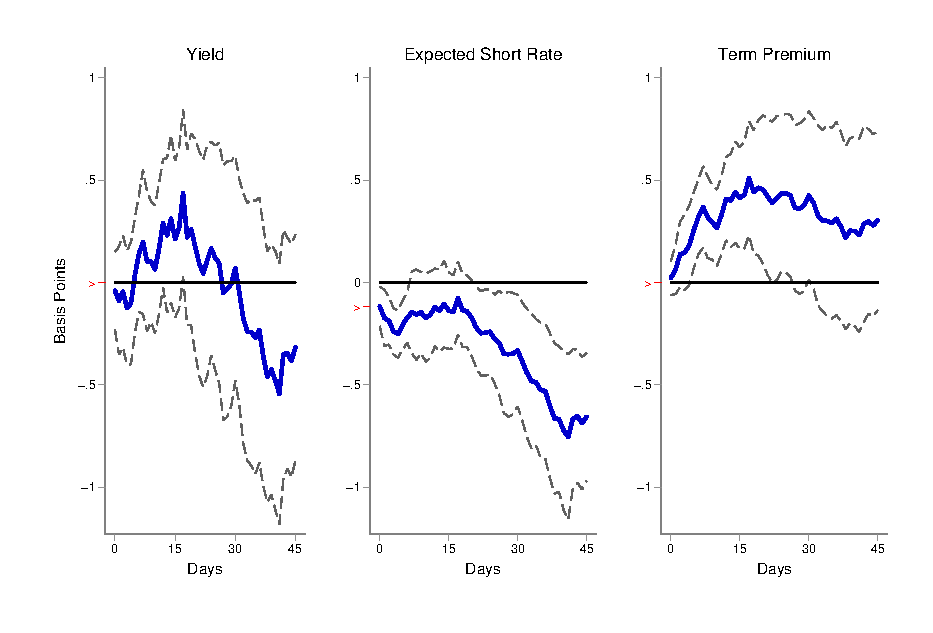
\includegraphics[trim={0cm 0cm 0cm 0cm},clip,height=0.35\textheight,width=\linewidth]{../Figures/LPs/LagDep-FX/Target/US/DCMP/TargetUSDnomyptp120m.eps} \\
						\vspace{-0.35cm}
						\caption{10-Year Yield} \label{subfig:LPUS10Ytarget}
						\vspace{0.4cm}
					\end{subfigure}
					
					\vspace{0.5cm}
					
					\begin{subfigure}[t]{\linewidth}
						\includegraphics[trim={0cm 0cm 0cm 0cm},clip,height=0.35\textheight,width=\linewidth]{../Figures/LPs/LagDep-FX/Target/US/DCMP/TargetUSDnomyptp24m.eps} \\
						\vspace{-0.35cm}
						\caption{2-Year Yield} \label{subfig:LPUS2Ytarget}
						\vspace{0.4cm}
					\end{subfigure}
				\end{center}
				\fignotes{This figure shows the response following \cite{Jorda:2005} of the 10- and 2-year U.S. yields and their components to a target surprise. The U.S. yield is the zero coupon yield from \cite{GSW:2007}. The yield is decomposed into an expected future short-term interest rate and a term premium following \cite{KimWright:2005}. Target surprises are identified using high-frequency data around Fed's monetary policy announcements, see section \ref{sec:USMPS} for details.}
			\end{minipage}
		\end{center}
	\end{figure}

	\pagebreak[4]
	
	\begin{figure}[tbph]
		\caption{Response of the U.S. Yield Curve to a Forward Guidance Surprise: 2000-2019} \label{fig:LPUSpath}
		\begin{center}
			\begin{minipage}{\linewidth}
				\begin{center}
					\begin{subfigure}[t]{\linewidth}
						\includegraphics[trim={0cm 0cm 0cm 0cm},clip,height=0.35\textheight,width=\linewidth]{../Figures/LPs/LagDep-FX/Path/US/DCMP/PathUSDnomyptp120m.eps} \\
						\vspace{-0.35cm}
						\caption{10-Year Yield} \label{subfig:LPUS10Ypath}
					\end{subfigure}
					
					\vspace{0.5cm}
					
					\begin{subfigure}[t]{\linewidth}
						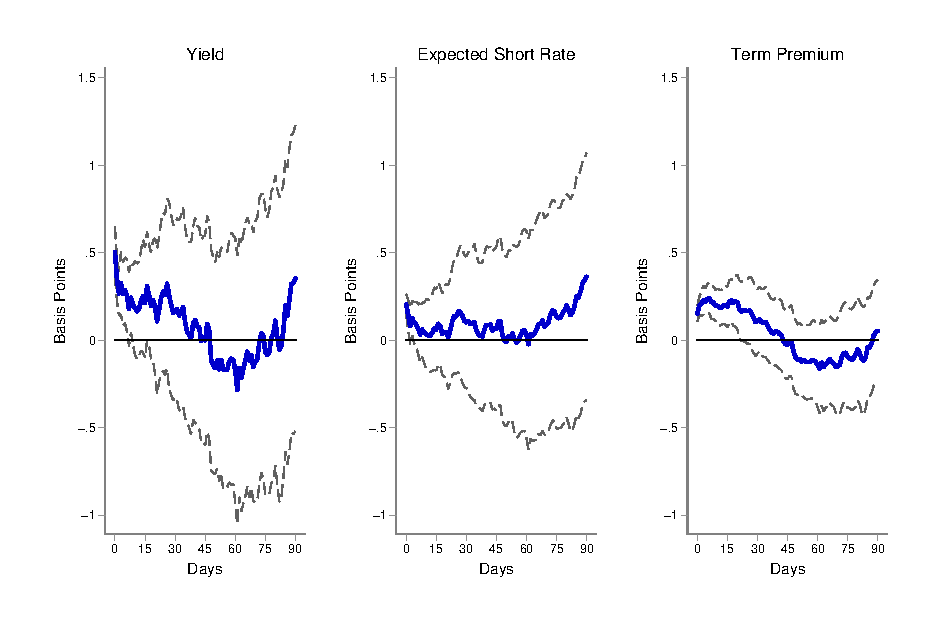
\includegraphics[trim={0cm 0cm 0cm 0cm},clip,height=0.35\textheight,width=\linewidth]{../Figures/LPs/LagDep-FX/Path/US/DCMP/PathUSDnomyptp24m.eps} \\
						\vspace{-0.35cm}
						\caption{2-Year Yield} \label{subfig:LPUS2Ypath}
					\end{subfigure}
				\end{center}
				\fignotes{This figure shows the response following \cite{Jorda:2005} of the 10- and 2-year U.S. yields and their components to a forward guidance surprise. The U.S. yield is the zero coupon yield from \cite{GSW:2007}. The yield is decomposed into an expected future short-term interest rate and a term premium following \cite{KimWright:2005}. Forward guidance surprises are identified using high-frequency data around Fed's monetary policy announcements, see section \ref{sec:USMPS} for details.}
			\end{minipage}
		\end{center}
	\end{figure}

	\pagebreak[4]
	
	\begin{figure}[tbph]
		\caption{Response of the U.S. Yield Curve to an Asset Purchase Surprise: 2009-2019} \label{fig:LPUSlsap}
		\begin{center}
			\begin{minipage}{\linewidth}
				\begin{center}
					\begin{subfigure}[t]{\linewidth}
						\includegraphics[trim={0cm 0cm 0cm 0cm},clip,height=0.35\textheight,width=\linewidth]{../Figures/LPs/LagDep-FX/LSAP/US/DCMP/LSAPUSDnomyptp120m.eps} \\
						\vspace{-0.35cm}
						\caption{10-Year Yield} \label{subfig:LPUS10Ylsap}
					\end{subfigure}
					
					\vspace{0.5cm}
					
					\begin{subfigure}[t]{\linewidth}
						\includegraphics[trim={0cm 0cm 0cm 0cm},clip,height=0.35\textheight,width=\linewidth]{../Figures/LPs/LagDep-FX/LSAP/US/DCMP/LSAPUSDnomyptp24m.eps} \\
						\vspace{-0.35cm}
						\caption{2-Year Yield} \label{subfig:LPUS2Ylsap}
					\end{subfigure}
				\end{center}
				\fignotes{This figure shows the response following \cite{Jorda:2005} of the 10- and 2-year U.S. yields and their components to an asset purchase surprise. The U.S. yield is the zero coupon yield from \cite{GSW:2007}. The yield is decomposed into an expected future short-term interest rate and a term premium following \cite{KimWright:2005}. Asset purchase surprises are identified using high-frequency data around Fed's monetary policy announcements, see section \ref{sec:USMPS} for details.}
			\end{minipage}
		\end{center}
	\end{figure}
\end{document}
% trim = {<left> <lower> <right> <upper>} % appendix
\documentclass{article}
\usepackage{graphicx}
\usepackage[margin=1in]{geometry}
\usepackage[outdir=./]{epstopdf}  					% Avoids errors when input figures
\usepackage[labelsep=period,labelfont=bf]{caption}
%\usepackage{subcaption}

\begin{document}
	\begin{figure}[tbph]
		\caption{Response of the U.S. Yield Curve to a Forward Guidance Surprise: 2000-2019} \label{fig:LPUSpathWh}
		\begin{center}
			\begin{minipage}{\linewidth}
				\begin{center}
					\begin{subfigure}[t]{\linewidth}
						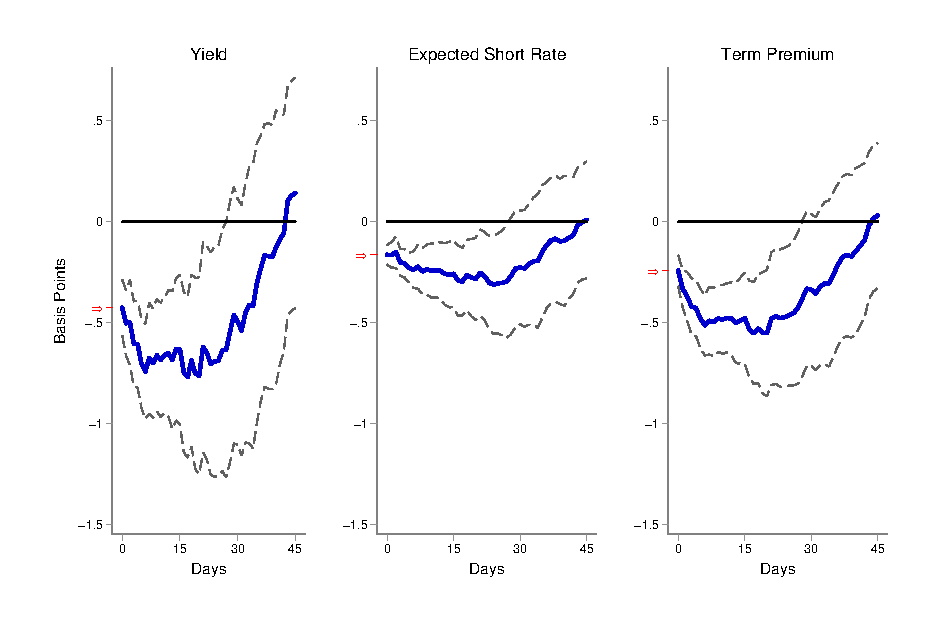
\includegraphics[trim={0cm 0cm 0cm 0cm},clip,height=0.35\textheight,width=\linewidth]{../Figures/LPs/LagDep-FX/Path/US/PathUSDnomyptp120m.eps} \\
						\vspace{-0.35cm}
						\caption{10-Year Yield} \label{subfig:LPUS10YpathWh}
					\end{subfigure}
					
					\vspace{0.2cm}
					
					\begin{subfigure}[t]{\linewidth}
						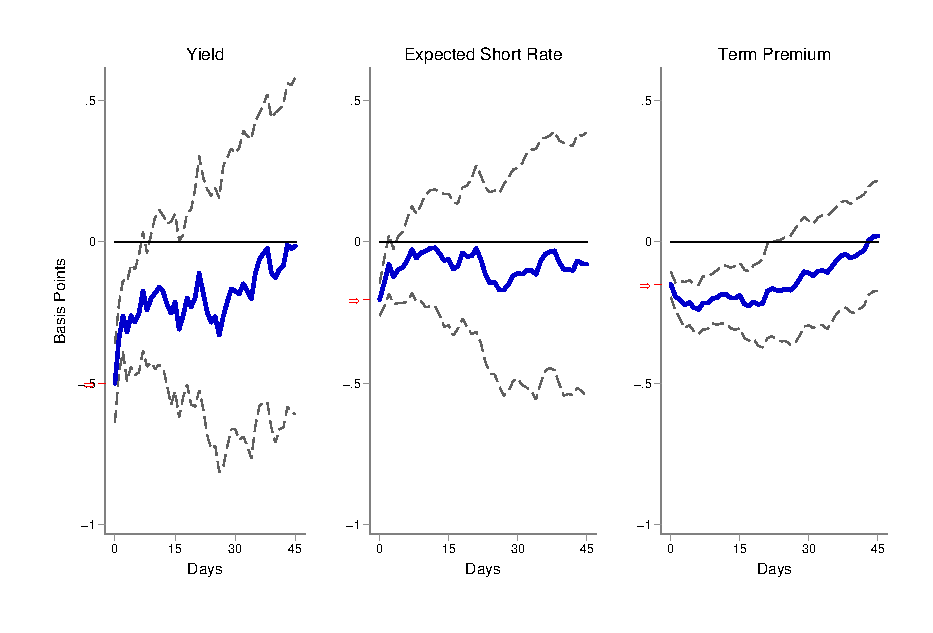
\includegraphics[trim={0cm 0cm 0cm 0cm},clip,height=0.35\textheight,width=\linewidth]{../Figures/LPs/LagDep-FX/Path/US/PathUSDnomyptp24m.eps} \\
						\vspace{-0.35cm}
						\caption{2-Year Yield} \label{subfig:LPUS2YpathWh}
					\end{subfigure}
					\vspace{-0.45cm}
				\end{center}
				\fignotes{This figure shows the response following \cite{Jorda:2005} of the 10- and 2-year U.S. yields and their components to a forward guidance easing surprise of 1 basis point. U.S. yields are zero-coupon yields from \cite{GSW:2007}, and are decomposed into an expected future short-term interest rate and a term premium following \cite{KimWright:2005}. Forward guidance surprises are identified using intraday data around Fed's monetary policy announcements, see section \ref{sec:USMPS} for details. An arrow indicates the contemporaneous (\(\idxh = 0\)) effect. The 90\% confidence bands are based on Driscoll--Kraay standard errors.}
			\end{minipage}
		\end{center}
	\end{figure}
\end{document}
% trim = {<left> <lower> <right> <upper>}
\documentclass{article}
\usepackage[margin=1in]{geometry}
\usepackage[outdir=./]{epstopdf}  					% Avoids errors when input figures
\usepackage[labelsep=period,labelfont=bf]{caption}
%\usepackage{subcaption}
\usepackage{graphicx}
%\graphicspath{{../Figures/LPs/LagDep-FX/Target/EM/}{../Figures/LPs/LagDep-FX/Path/EM/}{../Figures/LPs/LagDep-FX/LSAP/EM/}}

\begin{document}
	\begin{figure}[tbph]
		\caption{Response of the Emerging Market Yield Curve to a Forward Guidance Surprise: 2000-2019} \label{fig:LPEMpathWh}
		\begin{center}
			\begin{minipage}{\linewidth}
				\begin{center}
					\begin{subfigure}[t]{\linewidth}
						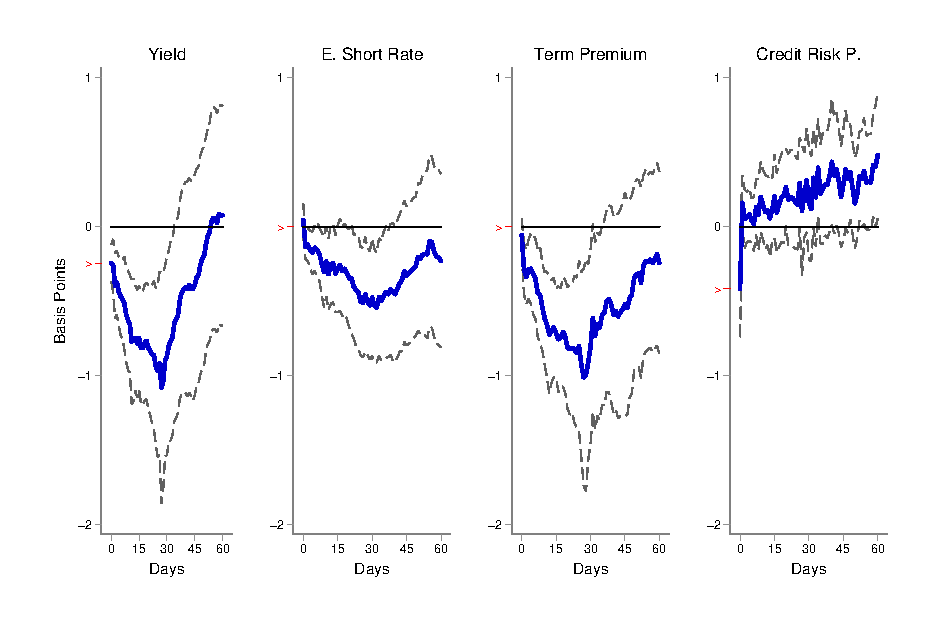
\includegraphics[trim={0cm 0cm 0cm 0cm},clip,height=0.35\textheight,width=\linewidth]{../Figures/LPs/LagDep-FX/Path/EM/PathEMnomyptpphi120m.eps} \\
						\vspace{-0.35cm}
						\caption{10-Year Yield} \label{subfig:LPEM10YpathWh}
					\end{subfigure}
					
					\vspace{0.2cm}
					
					\begin{subfigure}[t]{\linewidth}
						\includegraphics[trim={0cm 0cm 0cm 0cm},clip,height=0.35\textheight,width=\linewidth]{../Figures/LPs/LagDep-FX/Path/EM/PathEMnomyptpphi24m.eps} \\
						\vspace{-0.35cm}
						\caption{2-Year Yield} \label{subfig:LPEM2YpathWh}
					\end{subfigure}
					\vspace{-0.45cm}
				\end{center}
				\fignotes{This figure shows the response following \cite{Jorda:2005} of the 10- and 2-year emerging market nominal yields and their components to a forward guidance easing surprise of 1 basis point. Nominal yields are decomposed into an expected future short-term interest rate, a term premium and credit risk compensation, see section \ref{sec:Decomposition} for details. Forward guidance surprises are identified using intraday data around Fed's monetary policy announcements, see section \ref{sec:USMPS} for details. An arrow indicates the contemporaneous (\(\idxh = 0\)) effect. The 90\% confidence bands are based on Driscoll--Kraay standard errors.}
			\end{minipage}
		\end{center}
	\end{figure}
\end{document}
% trim = {<left> <lower> <right> <upper>}
\documentclass{article}
\usepackage{graphicx}
\usepackage[margin=1in]{geometry}
\usepackage[outdir=./]{epstopdf}  					% Avoids errors when input figures
\usepackage[labelsep=period,labelfont=bf]{caption}
%\usepackage{subcaption}

\begin{document}

% trim = {<left> <lower> <right> <upper>}

\begin{figure}[tbph]
	\caption{Response of the Forward Premium to U.S. Monetary Policy Shocks: EM}
	\label{fig:LPEMRHO}
	\begin{subfigure}[t]{\textwidth}
		\begin{center}
			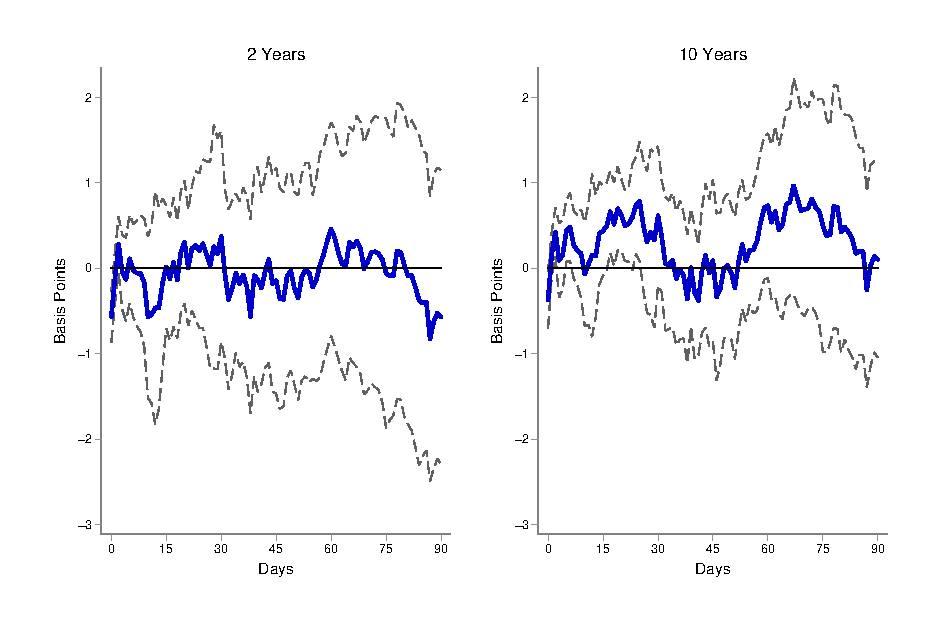
\includegraphics[trim={0cm 0cm 0cm 0cm},clip,height=0.26\textheight,width=1\textwidth]{../Figures/LPs/LagDep-FX/Target/EM/TargetEMrho.eps} \\
			\caption{Target Shock: 2000-2008} \label{subfig:LPEMRHOtarget}
%			\vspace{.5cm}
		\end{center}
	\end{subfigure}
	
	\begin{subfigure}[t]{\textwidth}
		\begin{center}
			\includegraphics[trim={0cm 0cm 0cm 0cm},clip,height=0.26\textheight,width=1\textwidth]{../Figures/LPs/LagDep-FX/Path/EM/PathEMrho.eps} \\
			\caption{Path Shock: 2000-2019} \label{subfig:LPEMRHOpath}
%			\vspace{.4cm}
		\end{center}
	\end{subfigure}
	
	\begin{subfigure}[t]{\textwidth}
		\begin{center}
			\includegraphics[trim={0cm 0cm 0cm 0cm},clip,height=0.26\textheight,width=1\textwidth]{../Figures/LPs/LagDep-FX/LSAP/EM/LSAPEMrho.eps} \\
			\caption{LSAP Shock: 2009-2019} \label{subfig:LPEMRHOlsap}
			%			\vspace{.4cm}
		\end{center}
	\end{subfigure}

%	\vspace{-0.4cm} \caption*{\footnotesize{\textit{Notes}: Notes.}}
\end{figure}

\pagebreak[4]

\begin{figure}[tbph]
	\caption{Response of the Forward Premium to U.S. Monetary Policy Shocks: AE}
	\label{fig:LPAERHO}
	\begin{subfigure}[t]{\textwidth}
		\begin{center}
			\includegraphics[trim={0cm 0cm 0cm 0cm},clip,height=0.26\textheight,width=1\textwidth]{../Figures/LPs/LagDep-FX/Target/AE/TargetAErho.eps} \\
			\caption{Target Shock: 2000-2008} \label{subfig:LPAERHOtarget}
			%			\vspace{.5cm}
		\end{center}
	\end{subfigure}
	
	\begin{subfigure}[t]{\textwidth}
		\begin{center}
			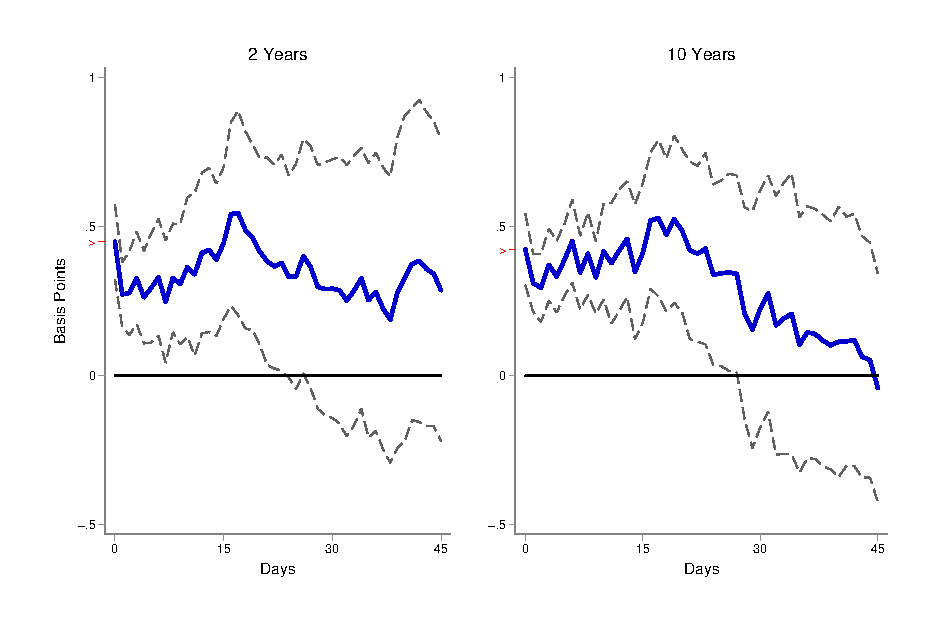
\includegraphics[trim={0cm 0cm 0cm 0cm},clip,height=0.26\textheight,width=1\textwidth]{../Figures/LPs/LagDep-FX/Path/AE/PathAErho.eps} \\
			\caption{Path Shock: 2000-2019} \label{subfig:LPAERHOpath}
			%			\vspace{.4cm}
		\end{center}
	\end{subfigure}
	
	\begin{subfigure}[t]{\textwidth}
		\begin{center}
			\includegraphics[trim={0cm 0cm 0cm 0cm},clip,height=0.26\textheight,width=1\textwidth]{../Figures/LPs/LagDep-FX/LSAP/AE/LSAPAErho.eps} \\
			\caption{LSAP Shock: 2009-2019} \label{subfig:LPAERHOlsap}
			%			\vspace{.4cm}
		\end{center}
	\end{subfigure}
	
	%	\vspace{-0.4cm} \caption*{\footnotesize{\textit{Notes}: Notes.}}
\end{figure}

\end{document}
 % appendix

\begin{landscape}
	\newpage
\end{landscape}

\end{appendices}